\documentclass[12pt]{article}
% Load packages
\usepackage{url}  % Formatting web addresses  
\usepackage{ifthen}  % Conditional 
\usepackage{multicol}   %Columns
\usepackage[utf8]{inputenc} %unicode support
\usepackage{amsmath}
\usepackage{amssymb}
\usepackage{epsfig}
\usepackage{epstopdf}
\usepackage{graphicx}
\usepackage[margin=0.1pt,font=footnotesize,labelfont=bf]{caption}
\usepackage{setspace}
%\usepackage{longtable}
\usepackage{colortbl}
%\usepackage{palatino,lettrine}
%\usepackage{times}
%\usepackage[applemac]{inputenc} %applemac support if unicode package fails
%\usepackage[latin1]{inputenc} %UNIX support if unicode package fails
\usepackage[wide]{sidecap}
%\usepackage[authoryear,round,comma,sort&compress]{natbib}
\usepackage[square,sort,comma,numbers]{natbib}
%\usepackage[authoryear,round]{natbib}
\usepackage{supertabular}
\usepackage{simplemargins}
\usepackage{comment}
\usepackage{lineno}

\urlstyle{rm}

%\textwidth = 6.50 in
%\textheight = 9.5 in
%\oddsidemargin =  0.0 in
%\evensidemargin = 0.0 in
%\topmargin = -0.50 in
%\headheight = 0.0 in
%\headsep = 0.25 in
%\parskip = 0.15in
%\linespread{1.75}
\doublespace

%\usepackage{geometry}
\usepackage{fullpage}

%\bibliographystyle{plain}
\bibliographystyle{msb}

\makeatletter
\renewcommand\subsection{\@startsection
	{subsection}{2}{0mm}
	{-0.05in}
	{-0.5\baselineskip}
	{\normalfont\normalsize\bfseries}}
\renewcommand\subsubsection{\@startsection
	{subsubsection}{2}{0mm}
	{-0.05in}
	{-0.5\baselineskip}
	{\normalfont\normalsize\itshape}}
\renewcommand\section{\@startsection
	{subsection}{2}{0mm}
	{-0.2in}
	{0.05\baselineskip}
	{\normalfont\large\bfseries}}	
\renewcommand\paragraph{\@startsection
	{paragraph}{2}{0mm}
	{-0.05in}
	{-0.5\baselineskip}
	{\normalfont\normalsize\itshape}}
\makeatother

%Review style settings
%\newenvironment{bmcformat}{\begin{raggedright}\baselineskip20pt\sloppy\setboolean{publ}{false}}{\end{raggedright}\baselineskip20pt\sloppy}

%Publication style settings

% Single space'd bib -
\setlength\bibsep{0pt}

\renewcommand{\rmdefault}{phv}\renewcommand{\sfdefault}{phv}

% Change the number format in the ref list -
\renewcommand{\bibnumfmt}[1]{#1.}

% Change Figure to Fig.
\renewcommand{\figurename}{Fig.}

% Begin ...
\begin{document}
\begin{titlepage}
{\par\centering\textbf{\Large Modeling and Analysis of Hormone and Mitogenic Signal Integration in Prostate Cancer}}
\vspace{0.05in}
{\par \centering \large{ Katharine V. Rogers, Joseph A. Wayman, Ryan Tasseff, Caitlin Gee, Matthew P. DeLisa, 
and Jeffrey D. Varner$^{*}$}}
\vspace{0.10in}
{\par \centering \large{School of Chemical and Biomolecular Engineering}}
{\par \centering \large{Cornell University, Ithaca NY 14853}}
\vspace{0.1in}
{\par \centering \textbf{Running Title:}~Modeling signal transduction in prostate cancer}
\vspace{0.1in}
{\par \centering \textbf{To be submitted:}~\emph{Molecular Systems Biology}}
\vspace{0.5in}
{\par \centering $^{*}$Corresponding author:}
{\par \centering Jeffrey D. Varner,}
{\par \centering Associate Professor, School of Chemical and Biomolecular Engineering,}
{\par \centering 244 Olin Hall, Cornell University, Ithaca NY, 14853} 
{\par \centering Email: jdv27@cornell.edu} 
{\par \centering Phone: (607) 255 - 4258}
{\par \centering Fax: (607) 255 - 9166}
\end{titlepage}
\date{}
\thispagestyle{empty}
\pagebreak
%%%%%%%%%%%%%%%%%%%%%%%%%%%%%%%%%%%%%%%%%%%%%%%%%%%%%%%%%%%%%%%%%%%%%%%%%%%%%%%%%%%%%%%%%%%%%%%%%%%%%%%%%%%
%%%%%%%%%%%%%%%%%%%%%%%%%%%%%%%%%%%%%%%%%%%%%%%%%%%%%%%%%%%%%%%%%%%%%%%%%%%%%%%%%%%%%%%%%%%%%%%%%%%%%%%%%%%
\section*{Abstract}
Prostate cancer is the most common cancer in men and the second leading cause of cancer related death in the United States. 
Androgens, such as testosterone, are required for prostate cancer growth. 
Androgen ablation in combination with radiation or chemotherapy remains the primary non-surgical treatment for androgen dependent prostate cancer. 
However, androgen ablation typically fails to permanently arrest cancer progression, often resulting in castration resistant prostate cancer (CRPC). 
CRPC is closely related to metastasis and decreased survival. 
In this study, we developed and analyzed a population of mathematical models describing growth factor and hormone signal integration in androgen dependent, intermediate and resistant prostate cancer cells. 
The model describes the integration of two simultaneous extracellular signaling inputs, namely, androgen and growth factors into a G1/S cell cycle checkpoint decision. 
Model parameters were identified from 43 studies in androgen dependent and resistant LNCaP cell lines. 
The model was validated by comparing simulations with an additional 29 data sets from LNCaP cell lines that were not used during training. 
Additionally, data from four drug trials was also used to evaluate the model’s performance.
Sensitivity analysis, conducted over an ensemble of prostate signaling models, suggested that in an androgen free environment general translation and transcription was more sensitive in androgen dependent cells, while in androgen independent cells the PI3K and MAPK pathway species were more sensitive. 
In a constant DHT environment sensitive species were conserved between the cell lines. 
These results suggest targeting the PI3K and MAPK pathways in addition to anti-androgen therapies as a treatment for CRPC.

\vspace{0.5in}
{\noindent \textbf{Keywords:}~Prostate cancer, signal transduction, mathematical modeling}

\pagebreak

\setcounter{page}{1}

\linenumbers

\section*{Introduction}

%
%Sipuleucel-T is a first generation cancer vaccine \cite{Kantoff2010}, while radium-223 is a targeted alpha emitter for bone metastasis \cite{Parker2013}. 
%Abiraterone is an inhibitor of cytochrome P450 17A1 (CYP17), a critical enzyme in androgen biosynthesis \cite{Sartor2013} while enzalutamide inhibits androgen receptor (AR) translocation to the nucleus, as well as DNA binding and coactivator recruitment \cite{Scher2012}.
%Thus, understanding the operation of the biological pathways which ultimately facilitate the transition to CRPC is vital to the discovery of new therapeutic strategies against this disease.
%The model focuses on the outlaw pathway, in which constitutively or overly-activated receptor tyrosine kinases (RTKs) stimulate AKT and mitogen-activated protein kinases (MAPKs), which in turn activate cytosolic androgen receptor (AR) in the absence of androgen. Interestingly, among the few genes activated AR represses is cellular prostatic acid phosphatase (cPAcP), itself a key regulatory of RTK activation. Thus, the outlaw pathway encodes crosstalk between RTK-dependent kinase and AR activation inside of a positive feedback loop. The model was validated with multiple experiments in LNCaP cell lines. In addition  For example, in response to enzalutamide, an AR inhibitor, the model predicted a decline in PSA expression similar to patient response.
%and there is limited data on combination therapies or the use of biomarkers to develop personalized treatment strategies. 

Prostate cancer (PCa) is the most commonly diagnosed cancer and the second leading cause of cancer-related death in men in the United States \cite{Siegel2013}. 
Initially, PCa cells depend upon the activation of cytosolic androgen receptors (AR) by androgen hormones, such as testosterone, for survival and growth. 
Androgen ablation in combination with radiation or chemotherapy remains the primary non-surgical treatment for androgen dependent prostate cancer (ADPC) \cite{Huggins1967}. 
However, androgen ablation typically fails to permanently arrest cancer progression as malfunctioning cells eventually lose androgen sensitivity and proliferate without hormone. 
The loss of androgen sensitivity results in castration resistant prostate cancer (CRPC), a phenotype closely linked with metastasis and greatly reduced survival \cite{Harris2009}.
Currently, there are six approved treatments that demonstrate a survival advantage in patients with metastatic CRPC, each of these target diverse aspects of the disease \cite{Sartor2013}.
The taxane family members docetaxel and cabazitaxel interact with microtubule stability \cite{Tannock2004,Bono2010}, while abiraterone \cite{Sartor2013} or enzalutamide \cite{Scher2012} interfere with androgen signaling by blocking androgen formation or nuclear translocation, respectively.
Other approved treatments are non-specific to PCa. 
For example, general treatments such as sipuleucel-T, a first generation cancer vaccine \cite{Kantoff2010}, 
and radium-223, an alpha emitter which targets bone metastasis \cite{Parker2013}, are both approved to treat CRPC.
Unfortunately, regardless of the therapeutic approach, the survival advantage of these treatments is typically only a few months. 
Thus, understanding the molecular basis of the loss of androgen sensitivity in CRPC could be an important step for the development of the next generation of therapies with a prolonged survival
advantage.   

Androgen-induced proliferation and survival depends upon many coordinated signal transduction and gene expression events. 
Androgen Receptor (AR) is part of the nuclear hormone receptor superfamily, which includes other important cancer targets such as progesterone receptor (PR) and estrogen receptor (ER) in breast cancer \cite{Aranda2001}. 
Nuclear hormone receptors act as ligand dependent transcription factors interacting with specific DNA sequences of target genes as either monomers, heterodimers, or homodimers; AR, PR, and ER act as homodimers. 
In the case of AR these specific DNA sequences are known as androgen response elements (ARE) \cite{Mangelsdorf1995}.
In the absence of androgen, AR is predominately found in the cytoplasm bound to heat shock proteins (HSP) \cite{Prescott2006}.
%Nuclear Hormone Receptors (Reviewed \cite{Aranda2001}) and AR in disease reviewed in \cite{Matsumoto2013}
Androgen, either testosterone or testosterone metabolites such as 5$\alpha$-dihydrotestosterone (DHT), enter prostate cells and interact with the cytosolic androgen receptor (AR). 
The interaction of DHT with AR promotes the dissociation of AR from chaperones such as HSP \citep{Pratt:1997kx} and its subsequent dimerization, phosphorylation and translocation to the nucleus (reviewed by Brinkmann \textit{et al.} \citep{Brinkmann1999}). 
Activated nuclear AR drives a gene expression program broadly referred to as androgen action, that promotes both proliferation and survival.
In addition to many genes including itself, activated nuclear AR promotes the expression and secretion of prostate specific antigen (PSA), arguably the best known PCa biomarker \citep{Feldman2001}.
PSA is commonly used as a prostate cancer indicator, although its prognostic ability is controversial \citep{Attard2009,Hoffman2011,Moyer2012}. 
In CRPC, AR signals in the absence of androgens. 
Androgen dependent (AD) prostate cells can become castration resistant (CR) through several possible mechanisms, including constitutively amplified AR expression and altered AR sensitivity to testosterone or other non-androgenic molecules \citep{Feldman2001}. 
In this study, we focused on the aberrant activation of AR by kinase signaling cascades, sometimes called the outlaw pathway. 
Outlaw pathway activation is driven by over-activated receptor tyrosine kinases (RTKs), a common pathology in many cancer types including PCa \citep{Slamon1989,Craft1999}. 
RTKs stimulate downstream kinases, including the AKT and mitogen-activated protein kinase (MAPK) pathways, which promote AR phosphorylation and dimerization in the absence of an androgen signal \citep{Craft1999,Yeh1999}. 
Interestingly, among the few genes activated AR represses is cellular prostatic acid phosphatase (cPAcP), itself a key regulatory of RTK activation \cite{Veeramani2005}. 
Thus, in CRPC the androgen program is initiated without the corresponding extracellular hormone cue, potentially from crosstalk between growth factor and hormone receptor pathways.

In this study, we developed a mathematical model of growth factor and hormone signal integration in androgen dependent, intermediate and resistant prostate cancer cells. 
We used this model to better understand which components and processes were differentially important in AD versus CR cells.
The new model architecture was a significant advance over our previous prostate signaling model \citep{Tasseff2010}. 
We added the regulated expression of ten additional proteins, including the cell cycle restriction point proteins cyclin D (and the differentially spliced variants cyclin D1a and cyclin D1b), cyclin E, cyclin-dependent kinase inhibitor 1A (p21Cip1), and cyclin-dependent kinase inhibitor 1B (p27Kip1). 
Also, we included the Rb/E2F pathway, expanded our description of the activation of the mammalian target of rapamycin (mTOR) protein and its role in translation initiation, and included the regulation of AR action by cyclin D1a and E2F. 
However, this upgraded architecture, while increasing the biological scope of the model, also expanded the number of unknown model parameters. 
To estimate these parameters, we used multiobjective optimization in combination with dynamic and steady-state data sets generated in AD, intermediate and CR LNCaP cell lines. 
We identified a population of approximately N = 5000 models (from well over a million candidate models) which described both AD and CR data sets using a single model structure.
Furthermore, we tested the model using an additional 29 LNCaP data sets not used for model training, along with four drug studies.
We analyzed the model population using sensitivity and robustness analysis to uncover differentially important mechanisms in AD versus CR cell lines. 
In the presence of androgen, the sensitivity profile was similar between AD and CR cells. 
Components of the MAPK and PI3K pathways were highly fragile, irrespective of the level of androgen dependence. 
However, in the absence of androgen, there were 609 statistically significant shifts in species sensitivity between AD and CR cells.
Of these, 108 were larger than one standard deviation above the mean.
In CR cells, HER2 activation of the MAPK and PI3K pathways was significantly more important, as was AR activation through the MAPK pathway. 
On the other hand, components of the translation and transcription infrastructure were differentially more important in AD cells in the absence of androgen.  
Taken together, our analysis suggested that independently targeting the PI3K or MAPK pathways in combination with anti-androgen therapies could perhaps be an effective treatment strategy for CRPC. 

%(323 more and 287 less sensitive)
%In this study, we rank-ordered the importance of the molecular components controlling the transition from ADPC to CRPC.
%Toward this, we developed and analyzed an ensemble of mechanistic mathematical models of the signal transduction processes governing the 
%transition from androgen dependent to castration resistant prostate cancer.
%The objective of this study was to rank-order the importance of components in CRPC and ADPC using computational tools. 
%We formulated and analyzed an ensemble of mechanistic mathematical models of the signal transduction processes in CRPC and ADPC 
%that was an extension of our previous work .
%In particular, we focused on the outlaw pathway and the possible crosstalk between RTK-dependent kinases and AR activation. 
%First, we expanded the original model by adding ten  
%Third, we added additional co-activators, such as cyclin E, and inhibitors of AR, such as
%ODE models typically contain a large number of unknown model parameters, which must be estimated  
%Due to uncertainty in parameter estimation and to account for differences between individual cells and cell sublines, an ensemble of parameter sets was used to model the system. 
%Proteins that were not modeled at a gene regulatory level were generated using zeroth order reactions. 
%All protein and RNA species were degraded with first order reaction rates. 
%To obtain an ensemble of parameter sets, we used multiobjective optimization. 
%Relative concentration values were quantified 
%Training data came from experiments on LNCaP sublines. 
%We used , previously developed in the lab \cite{Song2010}, to determine a diverse ensemble of models. 
%C-33 cells, having undergone fewer than 33 passages, are considered AD while C-51 cells, having between 34 and 80 passages, are considered an intermediate prostate cancer cell line. 
%C-81 (passage numbers beyond 80) display a CR phenotype \cite{Lin2000}. 
%http://endo.endojournals.org/content/140/11/5054.long or http://endo.endojournals.org/content/140/11/5054.long#ref-19

\clearpage

\section*{Results}

\subsection*{Estimating an ensemble of prostate signaling models.} 
We modeled the integration of growth factor, cell cycle and hormone signaling pathways in AD and CR LNCaP cells (Fig. \ref{fg:NetworkSchematic}). 
The signaling architecture was hand curated from over 80 primary literature sources in combination with biological databases.
The model equations were formulated as a system of ordinary differential equations (ODEs), where biochemical reaction rates were modeled using mass action kinetics.
ODEs and mass action kinetics are common modeling tools \citep{Wayman2013}, however, ODEs have the disadvantage of requiring estimates for unknown model parameters.
Many techniques have been developed to estimate ODE model parameters, often from noisy and sparse experimental data \citep{Moles:2003dn}.
Typically these identification problems are underdetermined, hence no unique parameter values can be estimated \citep{Villaverde:2014kl}.
Thus, instead of estimating a single yet highly uncertain parameter set, we estimated an ensemble of possible parameter sets using the Pareto Optimal Ensemble Techniques (POETs) algorithm \citep{Song2010}.
POETs uses a combination of simulated annealing and local optimization techniques coupled with Pareto optimality-based ranking to simultaneously optimize multiple objective functions.
Starting from an initial best fit set, we estimated the 1687 unknown model parameters (1674 kinetic parameters and 13 non-zero initial conditions) using 43 \textit{in vitro} data sets taken from AD, intermediate and CR LNCaP cells (Table~\ref{objective_table}). 
Each of the 43 training data sets was a separate objective in the multiobjective calculation. 
The training data were steady-state or dynamic immunoblots from which we extracted relative species abundance from their optical density profiles. 
POETs sampled well over a million possible parameter sets, from which we selected N = 5000 sets for further analysis. 
Over the ensemble, the coefficient of variation (CV) of the kinetic parameters spanned 0.59 - 5.8, with 33\% of the parameters having a CV of less than one (Fig. \ref{fg:Supp_CV}). 
As a control, we also performed simulations for R = 100 random parameter sets to compare against the ensemble generated by POETs. 

The ensemble of PCa models recapitulated training data in both AD and CR cell lines with only two experimentally justified parameter changes (Fig. \ref{fg:ColorPlot} and Fig. \ref{fg:Training}). 
Data from the LNCaP clones C-33 (dependent), C-51 (intermediate), and C-81 (resistant) \cite{Lin2000,Igawa2002,Horoszewicz1983} along with the CR LNCaP cell lines LNCaP-Rf \cite{Murillo2001}, LNCaP-AI \cite{Chen2011} and LNAI \cite{Graff2009} were used for model identification. 
To simulate the effective difference between LNCaP cell lines, the parameter controlling the maximum rate of PAcP gene expression was scaled by 0.1 and 0.5, respectively, for the C-81 and C-51 cell-lines compared to C-33. 
This modification was based upon steady-state PAcP data from the three LNCaP clones \cite{Lee2003}. 
Similarly, the expression of p16INK4 was adjusted in accordance with the study of Lu \textit{et al.} \citep{Lu1997}. 
These two parameters were the only adjustable parameter differences between AD and CR cells. 
To simulate an increased mTOR activation in the presence of a DHT stimulus, we added a first order activation term for mTOR activation with a DHT stimulus. Androgens have been shown to increase expression of proteins involved in cellular metabolism, which may lead to an increase in mTOR activation \cite{Xu2006}.
The model fit 36 of the 43 training objectives for greater than 40\% of the ensemble members (Fig. \ref{fg:ColorPlot}A). 
Conversely, only 10 of the 43 training objectives were captured with the random parameter control (Fig. \ref{fg:ColorPlot}B). 
The model captured the crosstalk between RTK activation and androgen action (Fig. \ref{fg:Training}). 
The model described DHT-induced PSA expression in both C-33 (Fig. \ref{fg:Training}A) and C-81 (Fig. \ref{fg:Training}B) cells. 
Interestingly, simulations with the HER2 inhibitor AG879 recapitulated decreased PSA expression in C-81 cells (Fig. \ref{fg:Training}C) in the absence of androgen stimulation.
AR action decreased the PAcP mRNA message (Fig. \ref{fg:Training}D), presumably leading to increased HER2 activity. 
The model also recapitulated the integration of androgen action with AR expression, G1/S cell cycle protein expression and AKT phosphorylation. 
For example, the model captured AR-induced AR expression following a DHT stimulus (Fig. \ref{fg:Training}H).
Conversely, the transcription factor E2F inhibits AR transcription in LNCaP cells (Fig. \ref{fg:Training}I). 
Other cell cycle proteins were also integrated with androgen action.
For example, the cyclin D1 abundance increased in CR compared to AD cells in the absence of androgen (Fig. \ref{fg:Training}E), while DHT induced p21Cip1 expression in C-33 cells (Fig. \ref{fg:Training}F).
The level of phosphorylated AKT was also increased in higher passage number cells (Fig. \ref{fg:Training}G). Taken together, [FINISH ME].

%We used a single model architecture to describe the behavior of both AD and CR LNCaP cells, 
%Two new additions to the model were the cell cycle protein p21Cip1 and transcriptional regulation of AR. 
%We were able to capture training data for both mechanisms. 
%AR transcriptionally upregulates its own expression \cite{Lin2003}\cite{Grad1999}. 
%We captured the increase in AR concentration due to AR activation, and thus increased transcriptional activity, upon  
%Higher basal AKT phosphorylation leads to increased activation of the PI3K/AKT pathway in PCa cells with less androgen dependence \cite{Lin2003}. 
%\cite{Davis2006}

%An additional protein we considered in validation that was present in training was phosphorylated SHC-transforming protein 1 (Shc).
%Simulations predicted a similar increase in Shc phosphorylation after DHT stimulus (Fig. \ref{fg:Validation}D) \cite{Veeramani2005Onc}. 
%The Prostate Cancer Working Group (PCWG) updated outcome measurements for castration resistant prostate cancer studies in 2008 \cite{Scher2008}. 
%The primary endpoint in prostate cancer studies is overall survival, while PSA response is often a secondary endpoint. 
%Figure \ref{fg:Validation}I shows fold change of PSA of ensemble members due to the application of sorafenib. 

%(Fig. \ref{fg:Validation}H)

\subsection*{Validation simulations revealed missing network structure.} 
The model was validated against 29 \textit{in vitro} and four \textit{in vivo} studies (Table~\ref{prediction_table}). 
For 15 of the 29 cases, greater than 40\% of the ensemble was qualitatively consistent with the experimental data (Fig. \ref{fg:ColorPlot}C). 
However, for the random parameter control, only 7 of the 29 cases were satisfied (Fig. \ref{fg:ColorPlot}D). 
We correctly predicted positive feedback between HER2 auto-activation and androgen action (Fig. \ref{fg:Validation}A and Fig. \ref{fg:Validation}B). 
We also captured the dose-dependence of AR abundance on DHT (Fig. \ref{fg:Validation}C). 
In addition to the cell line studies, we simulated the outcome of enzalutamide, lapatinib, and sorafenib clinical trials in AD and CRPC patients. 
The trial end points were the reduction in PSA expression relative to an untreated baseline.  
Enzalutamide acts on AR by inhibiting its nuclear translocation, DNA binding, and coactivator recruitment \cite{Scher2012}. 
In the enzalutamide trial, 54\% of the patients that received the drug showed a PSA decline of $\geq$ 50\% while 25\% showed a decline $\geq$ 90\%. 
We simulated enzalutamide exposure by reducing the rate constants governing activated AR binding to nuclear importer, cyclin E, and CDK6 to 1\% of their initial values. 
Consistent with the trial, 62\% of ensemble members showed a $\geq$ 50\% decline in PSA abundance, while 14\% showed a $\geq$ 90\% decline (Fig. \ref{fg:Validation}G). 
The second trial we simulated involved exposure of CRPC patients to sorafenib. 
Sorafenib is a kinase inhibitor with activity against Raf, vascular endothelial growth factor receptor (VEGFR), platelet-derived growth factor receptor (PDGFR), c-kit and c-Ret \cite{Dahut2008}. 
We considered only the effects of sorafenib on the protein kinase Raf, as VEGFR, PDGFR, c-kit and c-Ret were not included in the model. 
None of the 22 patients in the sorafenib study showed a PSA decline of $>$ 50\%. 
However, our simulations showed that approximately 55\% of the ensemble members had a PSA decline of $\geq$ 50\%. 
The last drug we considered was lapatinib, an inhibitor of epidermal growth factor receptor (EGFR) and HER2 tyrosine kinase activity \cite{Liu2013}. 
Two lapatinib drug trials were considered: one in which patients had CRPC and one in which patients had biochemically relapsed ADPC \cite{Whang2013,Liu2013}. 
In the CRPC lapatinib drug trial, two of the 21 enrolled patients had a PSA response $\geq$ 47\%  \cite{Whang2013}. 
For the CRPC case, our model showed 26.5\% of ensemble members with a PSA response $\geq$ 47\%. 
Of the 35 patients enrolled in the ADPC lapatinib study, no PSA decreases was observed \cite{Liu2013}. 
In this case, our model showed 9.2\% of ensemble members with a PSA response $\geq$ 50\%.
Although no response to lapatinib was seen in ADPC clinical trials, \textit{in vitro} AD LNCaP experiments showed decreased PSA expression in response to lapatinib, most notably with the addition of DHT \cite{Liu2005}. 

Validation and training failures suggested the original signaling architecture was missing critical components. 
Several of the failed training and validation simulations involved the response of the network to epidermal growth factor (EGF) stimulation. 
For example, Chen \textit{et al.} showed that HER2 phosphorylation increased within five minutes following EGF stimulation of LNCaP-AI cells \citep{Chen2011}. 
We predicted no connection between HER2 phosphorylation and EGF stimulation on this short timescale (Fig. \ref{fg:Validation}E). 
Interestingly, we initially neglected the heterodimerization of HER2 with other ErbB family members in order to simplify the model.
However, Chen \textit{et al.} suggested that HER2-EGFR heterodimerization could be an important factor in EGF-driven activation of HER2 \cite{Chen2011}. 
We tested this hypothesis by developing a new model that included HER2 and EGFR heterodimerization. 
We set the rate constants governing the assembly of HER2/EGFR heterodimers equal to EGFR homodimer assembly; all other parameters were unchanged.
This was a reasonable first approximation, as the affinity of HER2/EGFR heterodimerization and EGRF homodimerization is thought to be similar \cite{Hendriks2003}. 
With the inclusion of HER2-EGFR heterodimerization, we qualitatively fit the EGF-induced HER2 activation case and improved our training for experiments that involved an EGF stimulus, e.g., cyclin D mRNA and protein abundance following an EGF stimulus in C-33 cells (Fig \ref{fg:ColorPlot}A and C, white pixels).   

%in diverse environments (i.e., DHT, no DHT, drug) 
%Stimuli included the presence or absence of DHT, presence of therapeutics, and also EGF. 
%PIP3 recruits AKT and PDK1 to the membrane where PDK1 activates AKT \cite{Vivanco2002}. 
%Thus, the PIP3 and AKT interaction is required in the model for AKT phosphorylation to occur. 

\subsection*{Sensitivity analysis identified differentially important features of the prostate architecture.} 
We used sensitivity analysis to identify important signaling components in AD versus CR cells (Fig. \ref{fg:Sensitivity}). 
We calculated first order steady-state sensitivity coefficients under different stimuli for 500 parameter sets selected from the ensemble. 
Signaling components were rank-ordered based upon analysis of their sensitivity coefficient values. 
In the presence of DHT, the sensitivity profile was similar for AD versus CR cells, with only a few differences (Fig. \ref{fg:Sensitivity}B). 
The top 2\% of sensitive species, regardless of androgen dependence, involved components from the MAPK and PI3K pathways. 
In particular, activated Ras, Raf, phosphorylated MEK, as well as PIP3 localized AKT, phosphorylated AKT, and PI3K were sensitive in both AD and CR cells. 
Species involving PAcP and p16INK4 were more sensitive in AD cells, which was expected since the expression of these two proteins were the only parameters changed between AD and CR cells. 
Other species such as E2F, cyclin E, and DHT-activated AR were also more sensitive in AD cells. 
On the other hand, HER2-Grb2-Gab activation of PI3K and AKT inhibition of RAF were more sensitive in CR cells.

The importance of signaling components varied with androgen dependence in the absence of DHT (Fig. \ref{fg:Sensitivity}A). 
There were 609 statistically significant shifts in species sensitivity (318 more and 291 less sensitive) between CR and AD cells in a non-androgen environment. 
However, only 108 of these shifts were greater than one standard deviation above the mean. 
In CR cells, HER2 activation of ERK and PI3K was more sensitive, as was AR activation through the MAPK pathway. 
This was expected, as outlaw pathway activity was elevated in castration resistant cells. 
Species in the MAPK pathway were in general more sensitive in CR cells (128 out of 140 significant), with all forms of sPAcP more robust in CR cells.
On the other hand, infrastructure pathways encoding transcription and translation were more sensitive in AD cells.
PSA  and cyclin D1b (mRNA and mRNA complexes) were the only species involved in translation that were more robust in AD cells (14 out of 116).
The transcription factor, E2F was more fragile in AD cells, while the transcription factors ETS and AP1 were more robust. 
ETS and AP1 are activated by phosphorylated ERK, and ETS is also activated by active PKC \cite{Wilkinson2000,Lindemann2003}. 
E2F is deactivated through binding to Rb, which is deactivated by cyclin D1 and CDK phosphorylation \cite{Lapenna2009}. 
The model also included AP1 suppression of AR transcriptional activity (more sensitive in CR) \cite{Sato1997}, as well as inhibition of transcription of the AR gene by E2F (more sensitive in AD) \cite{Davis2006}.
Species in the PI3K pathway that were more fragile in AD cells included Rheb and TOR complexes. 
Interestingly, these species were included as the last step in the PI3K pathway prior to translation, with the phosphorylation of 4E-BP1 by TOR being considered the beginning of translation in this model. 
This again indicates that in the absence of DHT general translation is more fragile in AD cells. 

There was a large shift in sensitive species between an androgen and a non-androgen environment in both AD and CR cell lines (Fig. \ref{fg:Sensitivity}C and Fig. \ref{fg:Supp_Sensitivity}). 
Of the 664 statistically significant shifts in AD cells, 288 were more sensitive between androgen versus non-androgen environments. 
However, only 119 shifts were larger than one standard deviation above the mean. 
Unsurprisingly, AR activation through DHT binding, with and without coactivators, in a DHT environment was more sensitive, as was AR inhibition of PAcP transcription (repressed by AR in the model). 
Species further upstream, such as HER2 activation of the MAPK and PI3K/AKT pathways, were also more sensitive in a DHT environment. 
Cell cycle species that were more fragile in the presence of DHT, included complexes involving p21Cip1 and CDC25A.
In a non-androgen environment, basal transcription (68 out of 72) and translation (114 out of 120) were more fragile. 
Other fragile species in the absence of DHT included Rb, E2F, Sam68, cyclin D1a complexes, phosphatases in the MAPK pathway, Rheb complexes, and TOR complexes. 

We also considered the sensitivity of CR cells following the application of the AR inhibitor enzalutamide in the presence of DHT (Fig. \ref{fg:Sensitivity}D). 
Species which were more sensitive in an androgen environment with enzalutamide included cytosolic AR, cPAcP, and p21Cip1. 
As we would expect, AR species found in the nucleus and/or bound to coactivators, were more robust in the absence of enzalutamide. 
The top two percent of sensitive species with and without enzalutamide were conserved. 
In a CR cell, enzalutamide had no effect on the sensitivity of PI3K/AKT species as well as many MAPK species (ERK, Raf, and MEK). 
Next, we looked at the effect of enzalutamide on a CR cell in both a non-androgen and DHT environment (Fig. \ref{fg:Supp_Sensitivity}). 
More sensitive species in a non-androgen environment included dimerized HER2, ERK, and PAcP. 
Species which were more robust in the non-androgen environment included, AR activated by DHT, AKT, p70, and AR bound to HSP.
The results of our sensitivity analysis indicate that instead of inhibiting solely the AR pathway (enzalutamide), a combination therapy targeting the PI3K or MAPK pathways in addition to AR may be more effective.

\subsection*{Experimental results confirm the need for dual therapies in prostate cancer.} 

The results from our sensitivity analysis indicate that instead of inhibiting solely the AR pathway (enzalutamide), a combination therapy is necessary. 
To test this hypothesis we used the well characterized ADPC cell line LNCaP as well a LNCaP derived CRPC cell line C4-2 \cite{Thalmann1994}. 
Three inhibitors were used: the AR inhibitor MDV3100 (enzalutamide), the Raf kinase inhibitor sorafenib, and the PI3K inhibitor LY294002. 
In both cell lines, inhibition of either the AR or MAPK pathway appears to promote activation of the PI3K pathway, as seen by the increase in pAKT (S473) (Fig. \ref{fg:Experiment}A). 
The addition of the PI3K inhibitor, LY294002, alone or in combination diminishes PI3K activity. 
The inhibition of PI3K alone, led to an increase in AR expression in both LNCaP and C4-2 cell lines. 
Since, AR transcriptionally upregulates its own expression \cite{Lin2003}\cite{Grad1999}, this may indicate an increase in AR activity. 
The ribosomal protein pS6 was completely inhibited only in the presence of the PI3K inhibitor LY294002. 
Cell viability results show a large decrease in cell viability at 72 hrs in the dual inhibition cases as well as the triple inhibition case for both LNCaP and C4-2 cell lines (Fig. \ref{fg:Experiment}B). 
In both cell lines, MDV3100 (10 $\mu$M), has only a modest effect on cell viability versus control (DMSO). 
Figure \ref{fg:Experiment}C shows cell viability of both cell lines in varying concentrations of inhibitors at 24 hrs. 
  
  
\subsection*{Robustness analysis identified key regulators of prostate cancer.} 
Robustness analysis was conducted for 80 proteins to quantify the effects of amplifying or knocking down key model components in both AD and CR cells. 
Gene expression parameters were altered by a factor 10, 0.5, and 0 for knock-in, knock-down, or knock-out perturbations, respectively.
We calculated the effect of these perturbations on different protein markers, such as PSA, AR, and cyclin D. 
A knock-out of Raf, MEK or ERK showed an overall increase in cyclin D levels in CR cells (Fig. \ref{fg:Supp_Robustness}). 
This was unexpected and we saw a similar increase in cyclin D due to the knock-in of Raf, MEK or ERK. 
We found that individual ensemble members showed different response to a Raf knock-out, in both cyclin D concentration and PSA concentration. 
Of the 500 ensemble members, 126 members saw an increase in PSA concentration and 62 members saw an increase in cyclin D concentration due to the knock-out of Raf (Fig. \ref{fg:Robustness}). 
We saw three distinct regions: (1) increase in PSA concentration, (2) increase in cyclin D concentration, and (3) a decrease in both PSA and cyclin D. 
We explored the flux vectors of the outlying parameter sets to understand the mechanistic effect of Raf knock-out on PSA and cyclin D. 
Outlying parameter sets in region 1 displayed high activation of PI3K through HER2 signaling as well as high association of AP1 with AR. 
AP1 binds and suppresses AR transcriptional activity in LNCaP cells \cite{Sato1997}. 
Knocking out Raf lowered AP1 levels and, therefore, freed AR for increased transcription of PSA.
In region 2, parameter sets also had high activation of PI3K through HER2. 
They also had higher association of E2F with Rb and cyclin D1a with AR. 
Cyclin D levels in this region increase due to an increase in E2F levels caused by the Raf knock-out. 
Parameters in region 3 have high association of TOR. 
Interestingly, the drug sorafenib, a multi-kinase inhibitor that has activity against Raf, showed no measurable PSA decline in prostate cancer patients in clinical trials \cite{Dahut2008}. 
The robustness analysis showed that network perturbation can result in unexpected responses due to cell-to-cell heterogeneity in gene expression. 
These outlying cell types could be critical for understanding when designing drug targets and combination therapies.

%The results of the model suggest that an inhibition of either the PI3K pathway or the MAPK pathway in combination with an AR inhibitor as a possible therapy for CRPC. 
%Sensitivity analysis revealed no change in the top sensitive species in the presence or absence of the AR inhibitor, enzalutamide. PI3K/AKT and MAPK species continued to fall in the top two percent of sensitive species. 
%A study by Carver \textit{et al.} looked at dual inhibition of AR and PI3K signaling in LNCaP cells and in a Pten-deficient murine prostate cancer model \cite{Parker2013}. 
%Using both the PI3K inhibitor, BEZ235, and the AR inhibitor, MDV3100 (enzalutamide), the group saw a drastic decrease in the total number of cells. 
%Each inhibitor on it’s own had a much smaller effect on total cell number. 
%They saw an increase in the cell death marker, c-PARP, in the dual inhibition case. 
%The group hypothesized that AKT inhibition leads to increased AR signaling activity through increased protein concentrations of HER3. 
%On the other hand, AR inhibition leads to increased AKT activity due to the down regulation of PHLPP, a protein phosphatase that regulates AKT. 
%For simplicity, the HER3 pathway and also cell death were not included in the model. 
%Dual knock-out studies of PI3K and AR in our model show no additive effect on any cell cycle proteins through the dual knock-out. 
%The pathways in our model appear to be uncoupled and therefore no synergy is shown in the dual knock-out case. 
%This could indicate that the combined decrease in cell population is entirely due to cell death. 
%The Carver \textit{et al.} study did not consider cell cycle proteins or cell growth. 
%Our model does show a decrease in cell cycle proteins in the PI3K knock-out as well as in the dual knock-out case. 
%This result seems to be consistent with the decreased cell growth in the PI3K knock-out case which is not dependent on cell death, as c-PARP levels are low. 
%The decrease in cell cycle proteins is due to a decrease in general translation, including free eIF4E levels and activated 40S ribosome subunit. 
%The decrease in p70 (S6) activation due to inhibition of PI3K is shown in both the model and in the Carver \textit{et al.} study (Supplementary Figure), indicating this result is due to the PI3K pathway. 
%It would be interesting to repeat the experiment looking at cell cycle proteins and also performing the experiment in CR LNCaP cells, instead of AD cells. 



 
\section*{Discussion}
In this study, we developed a population of mathematical models describing growth factor and hormone signal integration in androgen dependent, intermediate and resistant prostate cancer cells. 
These models described the regulation of androgen receptor expression and activation through androgen binding as well as a ligand-independent, MAPK-driven mechanism referred to as the outlaw pathway. 
An ensemble of model parameters was estimated using 43 steady-state and dynamic data sets taken from androgen dependent, intermediate and independent LNCaP cell lines using multiobjective optimization. 
Further, we tested the predictive power of the model by comparing model predictions against 33 novel data sets (including four \textit{in vivo} drug studies) not used during model training. 
The model ensemble captured 84\% of the training data and 52\% of the validation data relative to 23\% and 24\% for a random control population. 
Interestingly, during the the initial round of parameter estimation, we identified several potentially missing structural components not present in the original connectivity. 
One such component, EGF-induced HER2/EGFR heterodimerization, was added to the current generation model. 
Inclusion of this structural component significantly improved both training and validation performance using the same rate constants as the EGFR-homodimer case (no additional parameter fitting). 
We then analyzed the population of signaling models, using both sensitivity and robustness analysis, to identify the critical components controlling network performance in a variety of conditions. 

%Hendrick's \textit{et al.} hypothesized that HER2 heterodimerization amplified signals by allowing just one molecule of EGF to activate two receptors \cite{Hendriks2003}. 
%In our case, we see an amplified cyclin D concentration due to an equal amount of EGF stimulus. %
%Model connectivity involving EGF and the downstream effect on AR and AR-regulated genes also came up as an open question. 
%Whether EGF downregulates or upregulates AR activity is debatable and the biology is still unknown \cite{Cai2009,Cinar2005,Lin2003,Lin2001PNAS, Hakariya2006,Gregory2004,Ponguta2008,Guo2006,Weber2004}. 
%The current model assumed no direct effect of EGF on AR, and instead we saw increased AR activity through increased HER2 activation. 
%Further studies will need to be done to update this section of the model. 

In addition, three of the validation cases involved the effect of EGF on AR and AR-activated genes, i.e., PSA. 
Cai \textit{et al.} showed decreased expression of endogenous AR as well as androgen-regulated PSA in AD LNCaP cells due to an EGF stimulus \cite{Cai2009}. 
Cinar \textit{et al.} also showed decreased AR protein expression due to EGF, an effect reversed by the mTOR inhibitor, Rapamycin \cite{Cinar2005}. 
Model simulations show either the opposite trend or no effect due to EGF stimulus (Fig. \ref{fg:Validation}F) \cite{Cinar2005}. 
These results suggest missing network structure. 
From additional literature searches, the inhibition of AR activation through EGF is still an open question, with many groups debating the biology involved, predominately in the PI3K/AKT pathway. 
Lin \textit{et al.} found that in low passage number LNCaP cells (C-33), AKT negatively regulates AR by destabilizing it and marking it for ubiquitylation. 
In high passage number LNCaP (C-81), AKT levels are high which contribute to AR stability and less degradation \cite{Lin2003}. 
Wen \textit{et al.} showed that HER2 could induce AKT activation and LNCaP cell growth in the presence and absence of androgen \cite{Wen2000}. 
Another study shows AKT phosphorylation of AR at S213 and S790 suppresses AR transactivation and AR-mediated apoptosis of LNCaP \cite{Lin2001PNAS}. 
The study from Cai \textit{et al.} showed the reduction in AR was not due to degradation or PI3K/AKT signaling, but instead was due to decreased AR mRNA levels \cite{Cai2009}. 
They found that AR protein levels in CR cells were not affected by EGF. 
Others though have found that PSA expression, even in C-81 cells, is decreased by EGF \cite{Hakariya2006}. 
In other prostate cell lines, EGF has been shown to increase AR transactivation \cite{Gregory2004,Ponguta2008}. 
The MAPK pathway, which is downstream of EGFR, may also enhance AR responses to low levels of androgen \cite{Guo2006,Weber2004}. 
Due to the discrepancies in the literature, experiments should be performed before adding additional network connectivity to the model.

The population of PCa models was analyzed using sensitivity analysis to identify key signaling components and processes in both AD and CR cells. 
There was very little difference between sensitive and robust components in AD versus CR cells in the presence of androgen. 
MAPK and PI3K pathway components were consistently ranked in the top 2\% of sensitive species in the presence of androgen for both AD and CR cells.
On the other hand, cell cycle species, such as cyclin D-CDK4/6 complexes bound to cell cycle inhibitors (p27Kip1, p21Cip1, p16INK4), were consistently robust. However, this profile changed considerably in the absence of androgen.
The activation of PI3K and ERK by HER2 dimerization and autophosphorylation was significantly more important in CR versus AD cells.
Interestingly, AR activation by ERK was also more sensitive in CR versus AD cells in the absence of androgen.
Lastly, although AR-regulated transcriptional processes were equally sensitive between the cell types, general translational and transcriptional components were more robust in CR versus AD cells.
This evidence supports the current theory that CR cells will still respond to androgen and, thus, AR is still an active target in therapeutic against CRPC \cite{Karantanos2013}. 
Supporting the argument that AR can be activated in the absence of androgens by MAPK activation \cite{Feldman2001}. 
Advanced prostate cancers often have higher levels of E2F and other transcription factors \cite{Davis2006}.
Interestingly, E2F was more sensitive in AD cells, while other transcription factors (ETS and AP1) were more robust. 
The drug enzalutamide had no effect on the top 2\% of sensitive species. 
Species in the PI3K/AKT and MAPK pathways in the presence of enzalutamide were still highly sensitive. 
The application of enzalutamide, increased sensitivity of AR species found outside of the nucleus as well as PAcP species.
Robustness analysis indicated diverse effects of Raf knock-out on PSA and cyclin D concentrations. 
Clinical studies of sorafenib, a multi-kinase inhibitor that has activity against Raf, showed increase PSA levels in patients \cite{Dahut2008}. 
Our results indicate that cell-to cell heterogeneity in gene expression can play a significant role in determining cell response. 
Thus, combination therapies need to be considered even in the case of a Raf knock-out. 

The results of the model suggest that an inhibition of either the PI3K pathway or the MAPK pathway in combination with an AR inhibitor as a possible therapy for CRPC. 
Sensitivity analysis revealed no change in the top sensitive species in the presence or absence of the AR inhibitor, enzalutamide. 
PI3K/AKT and MAPK species continued to fall in the top two percent of sensitive species. 
A study by Carver \textit{et al.} looked at dual inhibition of AR and PI3K signaling in LNCaP cells and in a Pten-deficient murine prostate cancer model \cite{Parker2013}. 
Using both the PI3K inhibitor, BEZ235, and the AR inhibitor, MDV3100 (enzalutamide), the group saw a drastic decrease in the total number of cells. 
Each inhibitor on it’s own had a much smaller effect on total cell number. They saw an increase in the cell death marker, c-PARP, in the dual inhibition case. 
The group hypothesized that AKT inhibition leads to increased AR signaling activity through increased protein concentrations of HER3. 
On the other hand AR inhibition leads to increased AKT activity due to the down regulation of PHLPP, a protein phosphatase that regulates AKT. 
For the simplicity of this model, the HER3 pathway and also cell death were not included in the model. 
Dual knock-out studies of PI3K and AR in our model show no additive effect on any cell cycle proteins through the dual knock-out. 
The pathways in our model appear to be uncoupled and therefore no synergy is shown in the dual knock-out case. 
This could indicate that the combined decrease in cell population is entirely due to cell death. 
The Carver \textit{et al.} study did not consider cell cycle proteins or cell growth. 
Our model does show a decrease in cell cycle proteins in the PI3K knock-out as well as in the dual knock-out case. 
This result seems to be consistent with the decreased cell growth in the PI3K knock-out case which is not dependent on cell death, as c-PARP levels are low. 
The decrease in cell cycle proteins is due to a decrease in general translation, including free eIF4E levels and activated 40S ribosome subunit. 
The decrease in p70 (S6) activation due to inhibition of PI3K is shown in both the model and in the Carver \textit{et al.} study ((Fig. \ref{fg:Supp_Figure_KO_new.pdf})), indicating this result is due to the PI3K pathway. 
Our results confirm the Carver \textit{et al.} study in that a dual inhibition of AR and PI3K signaling led to a more prominent decrease in cell viability then each of the inhibitors alone. 
We extended the study to look at the addition of a third inhibitor, sorafenib, that inhibits Raf kinase in the MAPK pathway.  

%It would be interesting to repeat the experiment looking at cell cycle proteins and also performing the experiment in CR LNCaP cells, instead of AD cells.  

%and  in the CR CWR-R1 prostate cell line.
%a steroid receptor coactivator family member along with other important AR coregulators such as 
%transcriptional intermediary factor 2 (TIF-2)

The PCa signaling architecture was assembled after extensive literature review and hand curation of the biochemical interactions.
However, there are a number of areas where model connectivity could be refined, e.g., the regulation of AR phosphorylation.
We assumed a single canonical activating AR phosphorylation site (S515), with ERK being the major kinase and PP2A or PP1 being the major phosphatases responsible for regulating this site.  
MAPK activation following EGF treatment increases AR transcription and cell growth, partially through AR phosphorylation on MAPK consensus site S515 \cite{Ponguta2008}.
However, there are at least 13 phosphorylation sites identified on AR, with phosphorylation at six of these being androgen induced \cite{Gioeli2012}. 
Moreover, other kinases such as AKT, protein kinase C (PKC) family members, as well as Src-family kinases can all phosphorylate AR in prostate cells \cite{Guo2006,Ponguta2008}. 
For example, AKT activation leads to AR  phosphorylation at both S213 and S791 (however, the role of these sites remains unclear) \cite{Wen2000,Lin2001PNAS,Taneja2005,Lin2003}.  
AKT effects on AR may also be passage number dependent, with AKT repressing AR transcription in low passage number cells and enhancing transcription in higher passage numbers \cite{Lin2003}. 
Androgen independent phosphorylation of AR by Src family kinases (not currently in model) at Y534 \cite{Guo2006} or by protein kinase C (PKC) family members at the consensus site S578 could also be important for understanding the regulation of AR activity. 
A second area we will revisit is the gene expression program associated with androgen action, and particularly the role of AR coregulators.
Currently, we included only two AR coactivators, cyclin E and CDK6 \cite{Yamamoto2000,Lim2005} and three corepressors AP1, Cdc25A, and cyclin D1a in the model \cite{Sato1997,Chiu2009,Petre-Draviam2003}. 
However, there are at least 169 proteins classified as potential AR coregulators \cite{Heinlein:2002qy,Heemers2007} with many of these being differentially expressed in malignant cells.
For example, the expression of steroid receptor coactivator-1 (Src-1) and transcriptional intermediary factor 2 (Tif-2), both members of the steroid receptor coactivator family, are elevated in prostate cancer \cite{Gregory2001,Gregory2004}. 
Src-1 is phosphorylated by MAPK and interacts directly with AR to enhance AR-mediated transcription \cite{Heemers2007}. 
Another class of potentially important AR coregulators are the cell cycle proteins Cdc25 and Rb.
Unlike Cdc25A, Cdc25B (not in the model) can act as an AR coactivator leading to enhanced AR transcription activity \cite{Ngan2003}. 
The Rb protein, in addition to being a key cell cycle regulator, has been shown to be an AR coactivator in an androgen-independent manner in DU145 cells \cite{Yeh1998}.
However, there is some uncertainty about the role of Rb as Sharma \textit{et al.} showed that Rb decreased AR activation in multiple prostate cancer cell lines and xenografts \cite{Sharma2010}. 
Forkhead proteins have also been shown to activate as well as repress AR function. 
In prostate cancer, AKT suppresses AFX/Forkhead proteins, which diminishes expression of AFX target genes, such as p27Kip1 \cite{Graff2000, Brunet1999, Medema2000, Takaishi1999}. 
Lastly, undoubtedly there are several other signaling axes important in PCa, such as cytokine or insulin- and insulin-like growth factor signaling \citep{Cardillo2003,Heinlein2004,Tam2007,Seaton2008}.
Understanding the pathways associated with these signals and how they relate to the current model, may give us a more complete picture of CR prostate cancer. 

%Lastly, with an extended model, it would be beneficial to include possible biomarkers for drug outcomes, as currently there is no biomarker that is used to select treatments for patients  \cite{Sartor2013}. 
                
\clearpage

\section*{Materials and Methods}

\subsection*{Prostate model signaling architecture.}
We modeled the expression, translation and post-translational modifications of key components of the signaling architecture.  
The model, which consisted of 780 protein, lipid or mRNA species interconnected by 1674 interactions, was a significant extension to our previous model \cite{Tasseff2010} in several important areas. 
First, we included well-mixed nuclear, cytosolic, membrane and extracellular compartments (including transfer terms between compartments).
Next, we expanded the description of growth factor receptor signaling, considering both homo- and heterodimer formation between ErbB family members and the role of cellular and secreted prostatic acid phosphatase (cPAcP and sPAcP, respectively).
Both forms of PAcP were included because cPAcP downregulates HER2 activity, while sPAcP promotes modest HER2 activation \cite{Veeramani2005}. 
Third, we expanded the description of the G1/S transition of the cell cycle (restriction point). 
The previous model used the abundance of cyclin D as a proliferation marker, but did not include other proteins or interactions potentially important to the restriction point.
Toward this shortcoming, we included cyclin E expression (and its role as a coregulator of androgen receptor expression), enhanced the description of cyclin D expression and the alternative splicing of cyclin D mRNA (including the role of the splice variants in androgen action), included the Rb/E2F pathway as well as E2F inhibition of androgen receptor expression \cite{Davis2006}, and the cyclin-dependent kinases cyclin-dependent kinase 4 (CDK4) and cyclin-dependent kinase 6 (CDK6). 
We also included key inhibitors of the restriction point including cyclin-dependent kinase inhibitor 1 (p21Cip1), cyclin-dependent kinase inhibitor 1B (p27Kip1), and cyclin-dependent kinase inhibitor 2A (p16INK4) \cite{Sherr1999}. 
Fourth, we enhanced the description of growth factor induced translation initiation.
One of the key findings of the previous model was that growth factor induced translation initiation was globally sensitive (important in both androgen dependent and independent conditions). 
However, the description of this important subsystem was simplified in the previous model. 
Here, we expanded this subsystem, using connectivity similar to previous study of Lequieu \textit{et al.} \cite{Lequieu:2011eu}, and re-examined the importance of key components of this axis, such as mammalian target of rapamycin (mTOR), phosphatidylinositide 3-kinase (PI3K) and AKT.  
Lastly, we significantly expanded the description of the role of androgen receptor. 
The previous model assumed constant AR expression, consistent with studies in androgen dependent and independent LNCaP sublines \cite{Lee2003}.
However, other prostate cancer cell lines vary in their AR expression \cite{Sobel2005}. 
Thus, to capture androgen signaling in a variety of prostate cancer cells, we included the transcriptional regulation governing androgen receptor expression, updated our description of the regulation of androgen receptor activity and androgen action (gene expression program driven by activated androgen receptor). 
At the expression level, we included AR auto-regulation in combination with the co-activators cyclin E and CDK6 \cite{Yamamoto2000,Lim2005}. 
We also assumed androgen receptor could be activated through androgen binding or a ligand-independent, MAPK-driven mechanism referred to as the outlaw pathway \cite{Feldman2001,Yeh1999}. 
We assumed a single canonical activating AR phosphorylation site (S515), with phosphorylated extracellular-signal-regulated kinase 1/2 (ppERK1/2) being the major kinase and protein phosphatase 2 (PP2A) or phosphoprotein phosphatase 1 (PP1) being the major phosphatases responsible for regulating this site. 
Finally, we modeled androgen receptor induced gene expression, including prostate specific antigen (PSA), cPAcP and p21Cip1.

%This description includes  were added to the model because of their importance in co-regulating AR transcription regulation activity in prostate cells . 
%With the addition of cell cycle proteins, we also included 
%only considered cyclin D as a cell marker and 
%In both models we considered nuclear hormone (AR) and transmembrane growth factor receptor (homo- and heterodimers of ErbB1/2) activation through both ligand-dependent and independent mechanisms. 
%The model investigated the activation of AR through androgen binding or a ligand-independent, MAPK-driven mechanism. 
%In addition to MAPK-dependent outlaw activation of AR, the model also included transcriptional activation via MAPK signaling \cite{Feldman2001,Yeh1999}. 
%The PI3K/AKT/mTOR pathway for translation initiation was also included in the model, as well as the regulated expression of PSA, cyclin D,  
%Thus, 
%The model of Tasseff \textit{et al.}  
%In order 
%Additionally, expression of transcription factors AP-1 and ETS were also added to the model. 
%Another significant addition to the model was the inclusion of a nuclear compartment separate from the cytosol, membrane and extracellular environments. 
%The prostate model was developed to determine the shift in important signaling components between CR and AD prostate cancer cells. 

\subsection*{Formulation and solution of the model equations.}
The prostate model was formulated as a coupled set of non-linear ordinary differential equations (ODEs):
\begin{equation}\label{asseassertain_massbalance}
\frac{d\mathbf{x}}{dt}=\mathbf{S}\cdot\mathbf{r}\left(\mathbf{x},\mathbf{k}\right)\qquad\mathbf{x}\left(t_{o}\right)=\mathbf{x}_{o}
\end{equation}
The quantity $\mathbf{x}$ denotes the vector describing the abundance of protein, mRNA, and other species in the model ($780\times 1$).
The stoichiometric matrix $\mathbf{S}$ encodes the signaling architecture considered in the model ($780\times 1674$).  
Each row of $\mathbf{S}$ describes a signaling component while each column describes a particular interaction.
The $(i,j)$ element of $\mathbf{S}$, denoted by $\sigma_{ij}$, describes how species $i$ is involved with interaction $j$. 
If $\sigma_{ij}>0$, species $i$ is produced by interaction $j$. Conversely, If $\sigma_{ij}<0$, then species $i$ is consumed in interaction $j$. 
Lastly, if $\sigma_{ij}=0$, then species $i$ is not involved in interaction $j$.
The term  $\mathbf{r}\left(\mathbf{x},\mathbf{k}\right)$ denotes the vector of interactions rates ($1674\times{1}$).
Gene expression and translation processes as well as all biochemical transformations were decomposed into simple elementary steps, 
where all reversible interactions were split into two irreversible steps (supplemental materials). 
We modeled each network interaction using elementary rate laws where all reversible interactions were split into two irreversible steps. 
Thus, the rate expression for interaction $q$ was given by:
\begin{equation}\label{eq-mass-action}
r_{q}\left(\mathbf{x},k_{q}\right)=k_{q}\prod_{j\in\left\{\mathbf{R}_{q}\right\}}x_{j}^{-\sigma_{jq}}
\end{equation}
The set $\left\{\mathbf{R}_{q}\right\}$ denotes reactants for reaction $q$, while $\sigma_{jq}$ denotes the stoichiometric coefficient (element of the matrix $\mathbf{S}$) governing species $j$ in reaction $q$. The quantity $k_{q}$ denotes the rate constant (unknown) governing reaction $q$.
Model equations were generated in the C-programming language using the UNIVERSAL code generator, starting from an text-based input file (available in supplemental materials). 
UNIVERSAL, an open source Objective-C/Java code generator, is freely available as a Google Code project (http://code.google.com/p/universal-code-generator/). 
Model equations were solved using the CVODE solver in the SUNDIALS library \cite{Hindmarsh2005} on an Apple workstation (Apple, Cupertino, CA; OS X v10.6.8).

We ran the model to steady-state before calculating the response to DHT or growth factor inputs.
The steady-state was estimated numerically by repeatedly solving the model equations and estimating the difference between subsequent time points:
\begin{equation}
\Vert\mathbf{x}\left(t+\Delta{t}\right) - \mathbf{x}\left(t\right)\Vert_{2}\leq\gamma
\end{equation}
The quantities $\mathbf{x}\left(t\right)$ and $\mathbf{x}\left(t+\Delta{t}\right)$ denote the simulated abundance vector at time $t$ and $t + \Delta{t}$, respectively.
The $L_{2}$ vector-norm was used as the distance metric, where $\Delta{t} = 100$ hr of simulated time and $\gamma$ = 0.001 for all simulations.

We estimated an ensemble of model parameter sets using the Pareto Optimal Ensemble Techniques (POETs) multiobjective optimization routine \cite{Song:2009dq,Song2010,Lequieu:2011eu}. 
POETs minimized the residual between model simulations and 43 separate training objectives taken from protein and mRNA signaling data generated in androgen dependent, intermediate and independent LNCaP cell lines (Table \ref{objective_table}). 
From these training objectives, POETs generated $>10^6$ candidate parameter vectors from which we selected N = 5000 Pareto rank-zero vectors for further analysis. 
The set-to-set correlation between selected sets was approximately 0.60, suggesting only modest similarity between ensemble members.
Approximately 33\%, or 560 of the 1674 parameters had a coefficient of variation (CV) of less than 1.0, where the CV ranged from 0.59 to 5.8 over the ensemble.
Details of the parameter estimation problem and POETs are given in the supplemental materials. 

\subsection*{Sensitivity and robustness analysis.}
Steady-state sensitivity coefficients were calculated for N = 500 parameter sets selected from the ensemble by solving the augmented kinetic-sensitivity equations \cite{Dickinson1976}:
\begin{equation}
	\begin{bmatrix}
		\mathbf{S}\cdot\mathbf{r}(\mathbf{x},\mathbf{k}) \\
		\mathbf{A}(t_s)\mathbf{s}_j + \mathbf{b}_j(t_s)
	\end{bmatrix} = \begin{pmatrix}
		\mathbf{0} \\
		\mathbf{0}
	\end{pmatrix}
	   \qquad j = 1,2,\dots,\mathcal{P}
\end{equation}
where
\begin{equation}
s_{ij}(t_s)= \left. \frac{\partial{x_i}}{\partial{k_j}} \right|_{t_s}
\end{equation} for each parameter set.
Steady-state was calculated as described previously.
The quantity $j$ denotes the parameter index, $\mathbf{A}$ denotes the Jacobian matrix, and $\mathcal{P}$ denotes the number of parameters in the model. 
The vector $\mathbf{b}_j$ denotes the $j$th column of the matrix of first-derivatives of the mass balances with respect to the parameters. 
Steady-state sensitivity coefficients were used because of the computational burden associated with sampling several hundred parameters sets for each of the 1674 parameters. 
The steady-state sensitivity coefficients $\mathcal{N}_{ij} \equiv s_{ij}$ were organized into an array for each parameter set in the ensemble: 
\begin{equation}
	\mathcal{N}^{\left(\epsilon\right)} = 
	\begin{pmatrix}
		\mathcal{N}_{11}^{\left(\epsilon\right)} & \mathcal{N}_{12}^{\left(\epsilon\right)} & \hdots & \mathcal{N}_{1j}^{\left(\epsilon\right)} & \hdots & \mathcal{N}_{1P}^{\left(\epsilon\right)} \\
		\mathcal{N}_{21}^{\left(\epsilon\right)} & \mathcal{N}_{22}^{\left(\epsilon\right)} & \hdots & \mathcal{N}_{2j}^{\left(\epsilon\right)} & \hdots & \mathcal{N}_{2P}^{\left(\epsilon\right)} \\
		\vdots & \vdots & & \vdots & & \vdots \\
		\mathcal{N}_{M1}^{\left(\epsilon\right)} & \mathcal{N}_{M2}^{\left(\epsilon\right)} & \hdots & \mathcal{N}_{Mj}^{\left(\epsilon\right)} & \hdots & \mathcal{N}_{MP}^{\left(\epsilon\right)} \\
	\end{pmatrix}\qquad\epsilon = 1,2,\hdots,N_{\epsilon}
\end{equation}
where $\epsilon$ denotes the index of the ensemble member, $P$ denotes the number of parameters, $N_{\epsilon}$ denotes the number of parameter sets sampled (N = 500) and $M$ denotes the number of model species. 
To estimate the relative fragility or robustness of species and reactions in the network, we decomposed $\mathcal{N}^{\left(\epsilon\right)}$ 
using Singular Value Decomposition (SVD):

\begin{equation}
	\mathcal{N}^{\left(\epsilon\right)} = \mathbf{U}^{\left(\epsilon\right)}\Sigma^{\left(\epsilon\right)}\mathbf{V}^{T,{\left(\epsilon\right)}}
\end{equation}
Coefficients of the left singular vectors corresponding to largest $\theta$ $\leq$ 15 singular values of $\mathcal{N}^{\left(\epsilon\right)}$ were rank-ordered to estimate important species combinations, while coefficients of the right singular vectors were used to rank important reaction combinations. 
Only coefficients with magnitude greater than a threshold ($\delta$ = 0.001) were considered. 
The fraction of the $\theta$ vectors in which a reaction or species index occurred was used to quantify its importance (sensitivity ranking). 
We compared the sensitivity ranking between different conditions to understand how control in the network shifted in different cellular environments.  

Robustness coefficients were calculated as shown previously \cite{Tasseff2011}. 
Robustness coefficients denoted by $\alpha\left(i,j,t_{o},t_{f}\right)$ are defined as:
\begin{equation}
\alpha\left(i,j,t_{o},t_{f}\right)=\left(\displaystyle\int_{t_{o}}^{t_{f}}x_{i}\left(t\right)dt\right)^{-1}\left(\displaystyle\int_{t_{o}}^{t_{f}}x^{(j)}_{i}\left(t\right)dt\right)
\end{equation}
Robustness coefficients quantify the response of a marker to a structural or operational perturbation to the network architecture.
Here $t_o$ and $t_f$ denote the initial and final simulation time respectively, while $i$ and $j$ denote the indices for the marker and the perturbation respectively. 
A value of $\alpha\left(i,j,t_{o},t_{f}\right)>1$, indicates increased marker abundance, while $\alpha\left(i,j,t_{o},t_{f}\right)<1$ indicates decreased marker abundance following perturbation $j$. 
If $\alpha\left(i,j,t_{o},t_{f}\right)\sim{1}$ the $j$th perturbation does not influence the abundance of marker $i$.
Robustness coefficients were calculated (starting from steady-state) from $t_{o} = 0$ hr to $t_{f} = 72$ hr following the addition of 10nM DHT at $t_{o}$.
Robustness coefficients were calculated for the same N = 500 models selected for sensitivity analysis. 

\subsection*{Experimental Validation.}

\subsection*{Cell culture and treatments}
Androgen dependent LNCaP prostate cancer cells were a gift from Dr. Brian Kirby (Cornell University), and the Castrate Resistant C4-2 prostate cancer cell line was purchased from MD Anderson Cancer Center, University of Texas. Cell lines were maintained in RPMI 1640 media (Life Technologies, Inc., Grand Island, NY) with 10\% fetal calf serum (FBS; Hyclone) and 1x antibiotic/antimycotic (Sigma, St. Louis, MO) in a 5\% CO$_2$ humidified atmosphere at 37$^{\circ}$C. The AR inhibitor MDV3100 (enzalutamide) and the Raf inhibitor sorafenib were purchased from SantaCruz Biotechnology (Santa Cruz, CA). The PI3K inhibitor LY294002 was purchased from Cell Signaling Technologies (Danvers, MA, USA). All stock solutions were diluted in DMSO (Sigma, St. Louis, MO). 

\subsection*{Protein Extraction and Western Blot}

LNCaP and C4-2 cells were seeded in 60 mm dishes at a density of 4 x 10$^{5}$. After 96 and 72 hrs, for LNCaP and C4-2 cells respectively, the media was replaced with fresh media and drug treatments were added. After 24 hours, cells were washed twice in PBS buffer, scraped in 250 $\mu$L ice-cold lysis buffer (Pierce, Rockford, IL) supplemented with protease and phosphatase inhibitors (Sigma, St. Louis, MO), and lysed for 30 min on ice. Lysates were centrifuged at 13,000 rpm for 30 min at 4$^{\circ}$C. After quantification of total protein by BCA assay, equal amounts of total protein lysates (25 $\mu$g) were resolved by SDS-PAGE and transferred onto PVDF membranes. Membranes were blocked in 5\% fat free milk and then probed with antibodies. The primary antibodies used for western blot analysis were pAKT Ser473, AKT, pS6 Ser240/244 , pERK Thr202/Tyr204, ERK, AR, and GAPDH were from Cell Signaling Technologies (Danvers, MA, USA). For detection, enhanced chemiluminescence ECL reagent (GE Healthcare, Pittsburgh, PA) was used and signals were visualized using the ChemiDoc XRS system (Bio-Rad). 

\subsection*{MTT Assay}

LNCaP and C4-2 cells were seeded at a density of 1x10$^{4}$ cells per well in 96 well plates. After 48 hrs the media was refreshed and drug treatments added. Cell growth at 24, 48, and 72 hrs was determined using a 3-(4,5-dimethyl thiazol-2-yl)-2,5-diphenyl tetrazolium bromide (MTT) assay. At the specified time point 10 $\mu$L MTT reagent (stock of 5 mg/mL in PBS) was added to each well and the cells were further incubated for 4 hrs. At 4 hrs, the media was removed and 50 $\mu$L of dissolving reagent DMSO was added to each well. After an additional 10 min incubation, the absorbance was measured at 540 nm on a microplate reader. Each reading was adjusted by subtracting the absorbance value for the blank (media only) and the results were then scaled to the DMSO-treated (control) case. 


\section*{Acknowledgements}
This study was supported by award number U54CA143876 from the National Cancer Institute.
The content is solely the responsibility of the authors and does not necessarily represent the official views of the National Cancer Institute or the National Institutes of Health.
The authors acknowledge the financial support of the National Science Foundation, award no. DGE-1045513,for a GK12 training grant entitled "Grass Roots: Advancing Education in Renewable Energy and Cleaner Fuels through collaborative graduate fellow/teacher/grade-school student interactions."
We would like to thank Timothy Chu, Kyriakos Tsahalis, Spencer Davis, Rohit Yallamraju, Gongcheng Lu, and Yalin Zhao. 

\clearpage
%\bibliographystyle{plain}
%\bibliographystyle{IEEEbib}

\bibliography{References_v1}

%\begin{comment}

\clearpage

\begin{figure}\centering
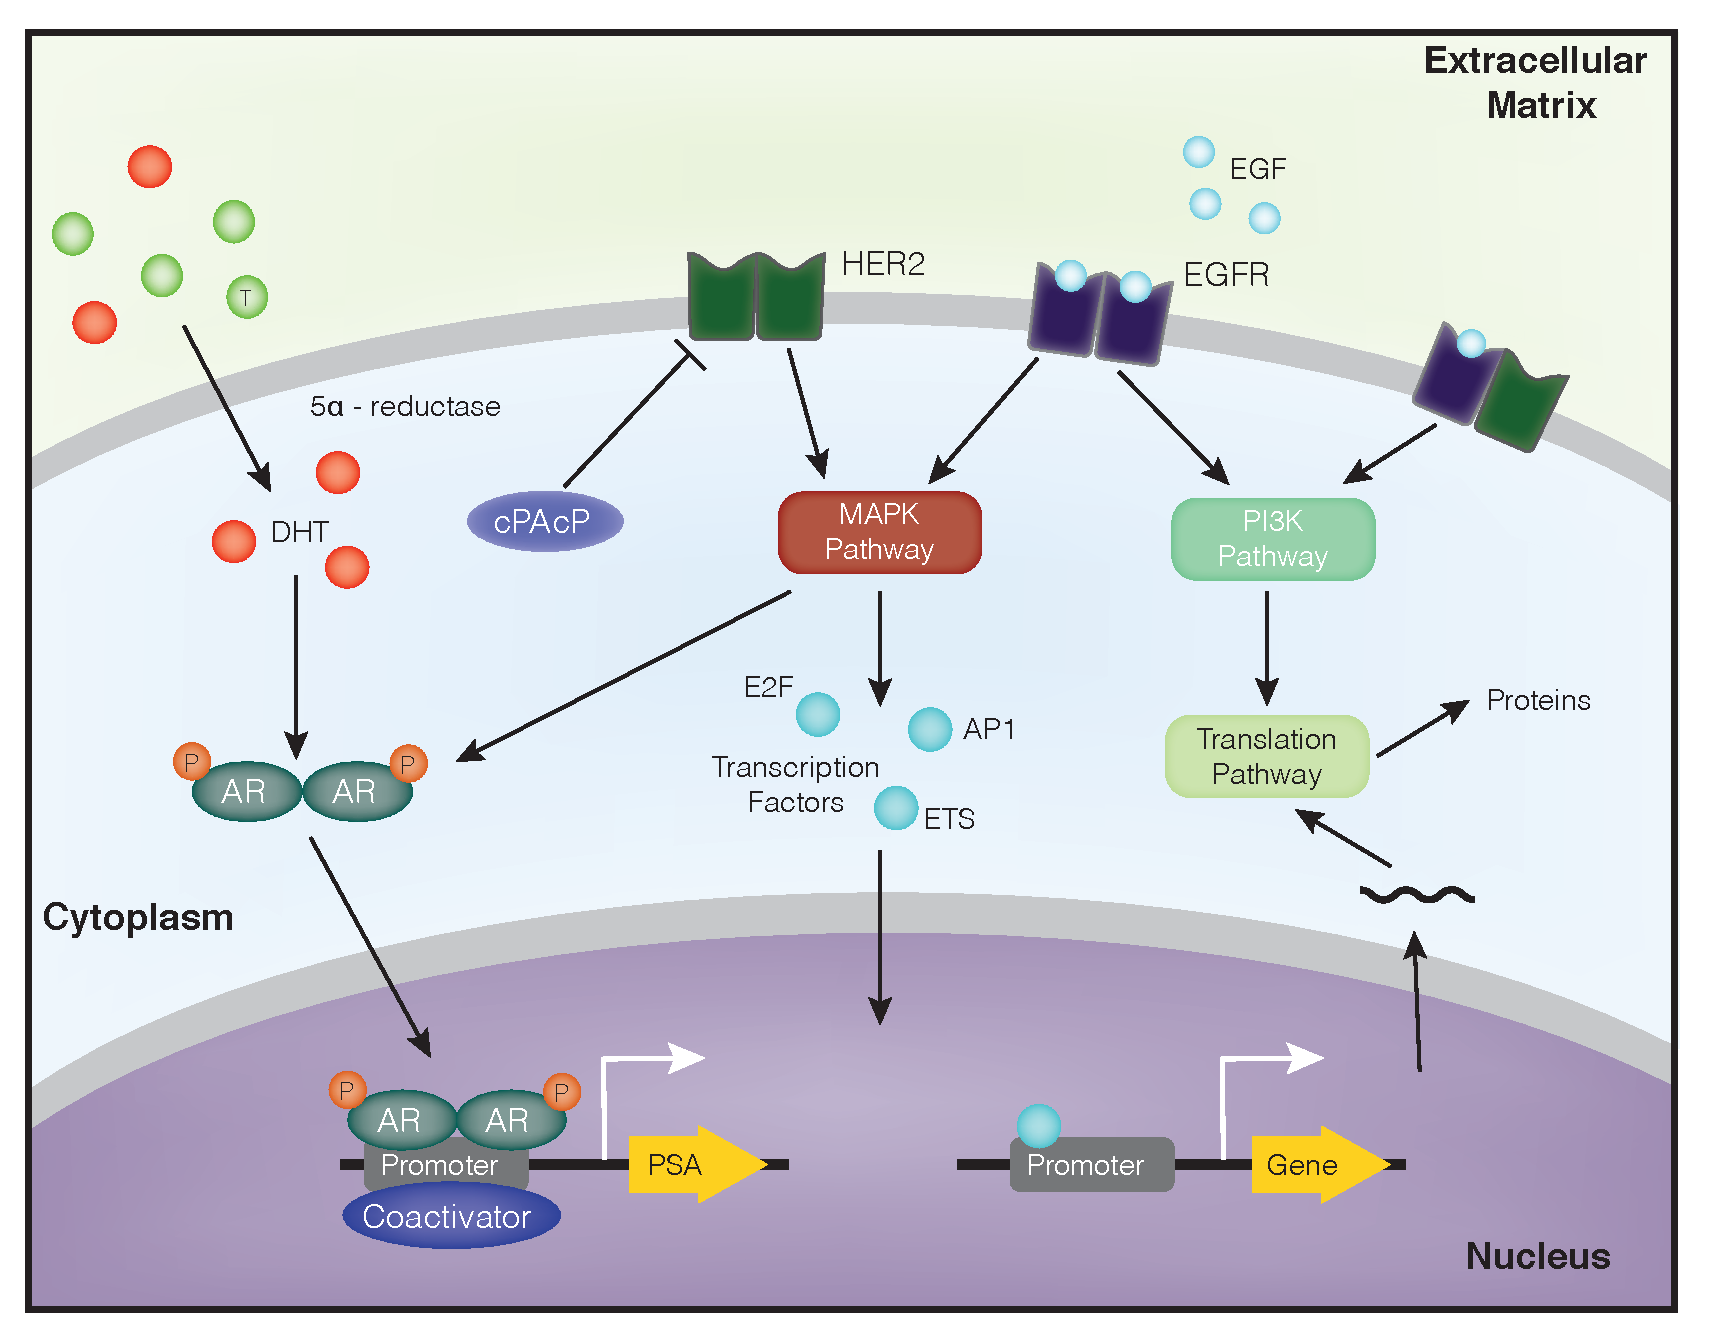
\includegraphics[width=1.0\textwidth]{./figs/Fig_1_LNCAPModel.pdf}
\caption{Schematic overview of the prostate signaling network. The model describes hormone and growth factor induced expression of several proteins, including PSA. In the absence of outside hormones/growth factors, overactive HER2 can stimulate the MAPK and AKT pathways. AR can be activated directly by the MAPK pathway.
}
\label{fg:NetworkSchematic}
\end{figure}

\clearpage

\begin{figure}\centering
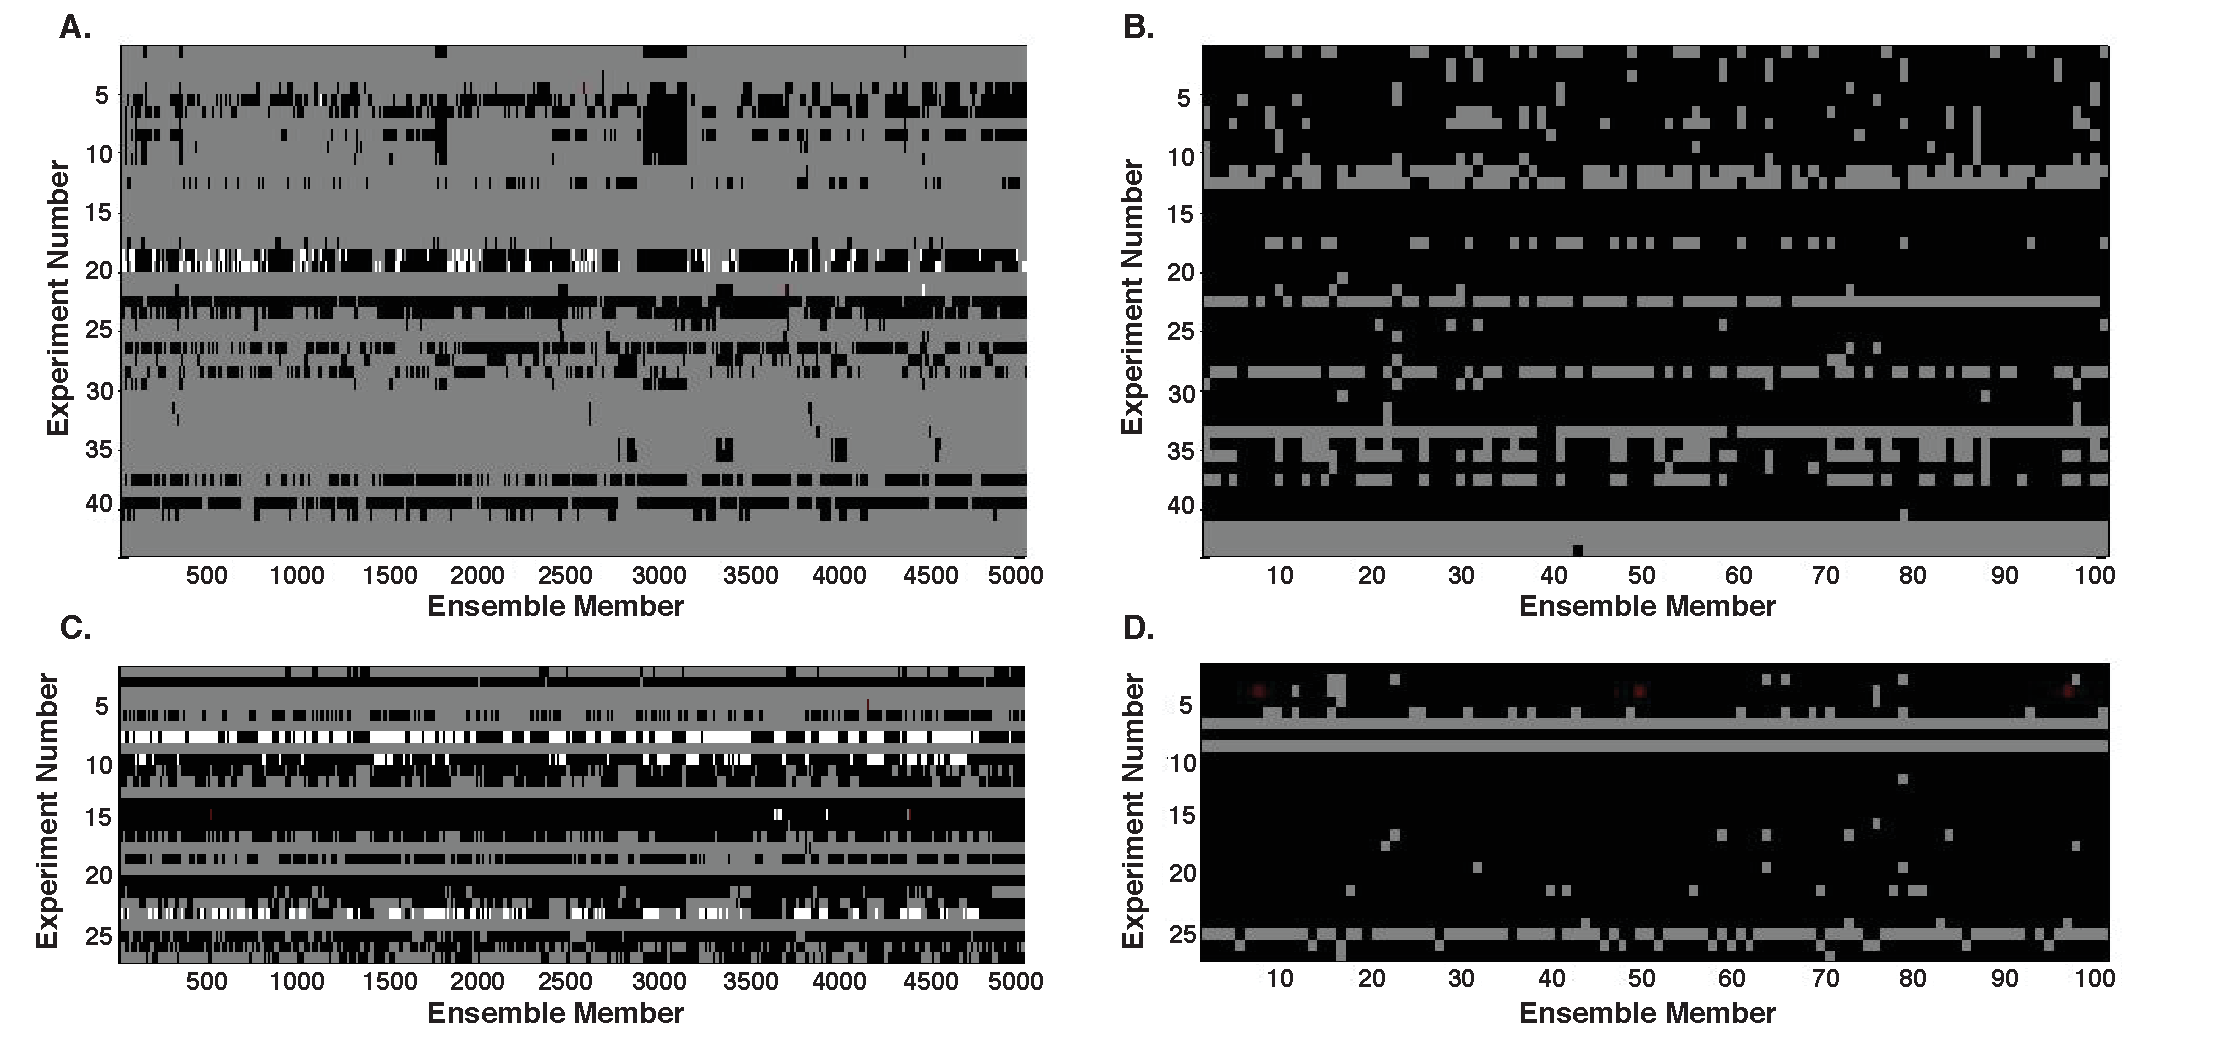
\includegraphics[width=1.0\textwidth]{./figs/Fig_3_ColorPlot.pdf}
\caption{Simulation results versus experimental results for training and validation data. Experiment numbers 1 through 43 were used for training, while experiments 44 through 72 were validation. Gray means the ensemble member qualitatively fit experimental data in both models. White means the the ensemble member only fit the data using the new model that included HER2 heterodimerization. Red means the ensemble member fit using only the old model. Black corresponds to an incorrect cellular response in both models.   $\bf{A.,C.}$ Training and validation results, respectively, for entire ensemble population using both the original model and an updated model including HER2 heterodimerization (N = 5000). $\bf{B.,D.}$ Simulation results for training and validation of a random set of 100 members using both models. 
 }
\label{fg:ColorPlot}
\end{figure}

\clearpage

\begin{figure}\centering
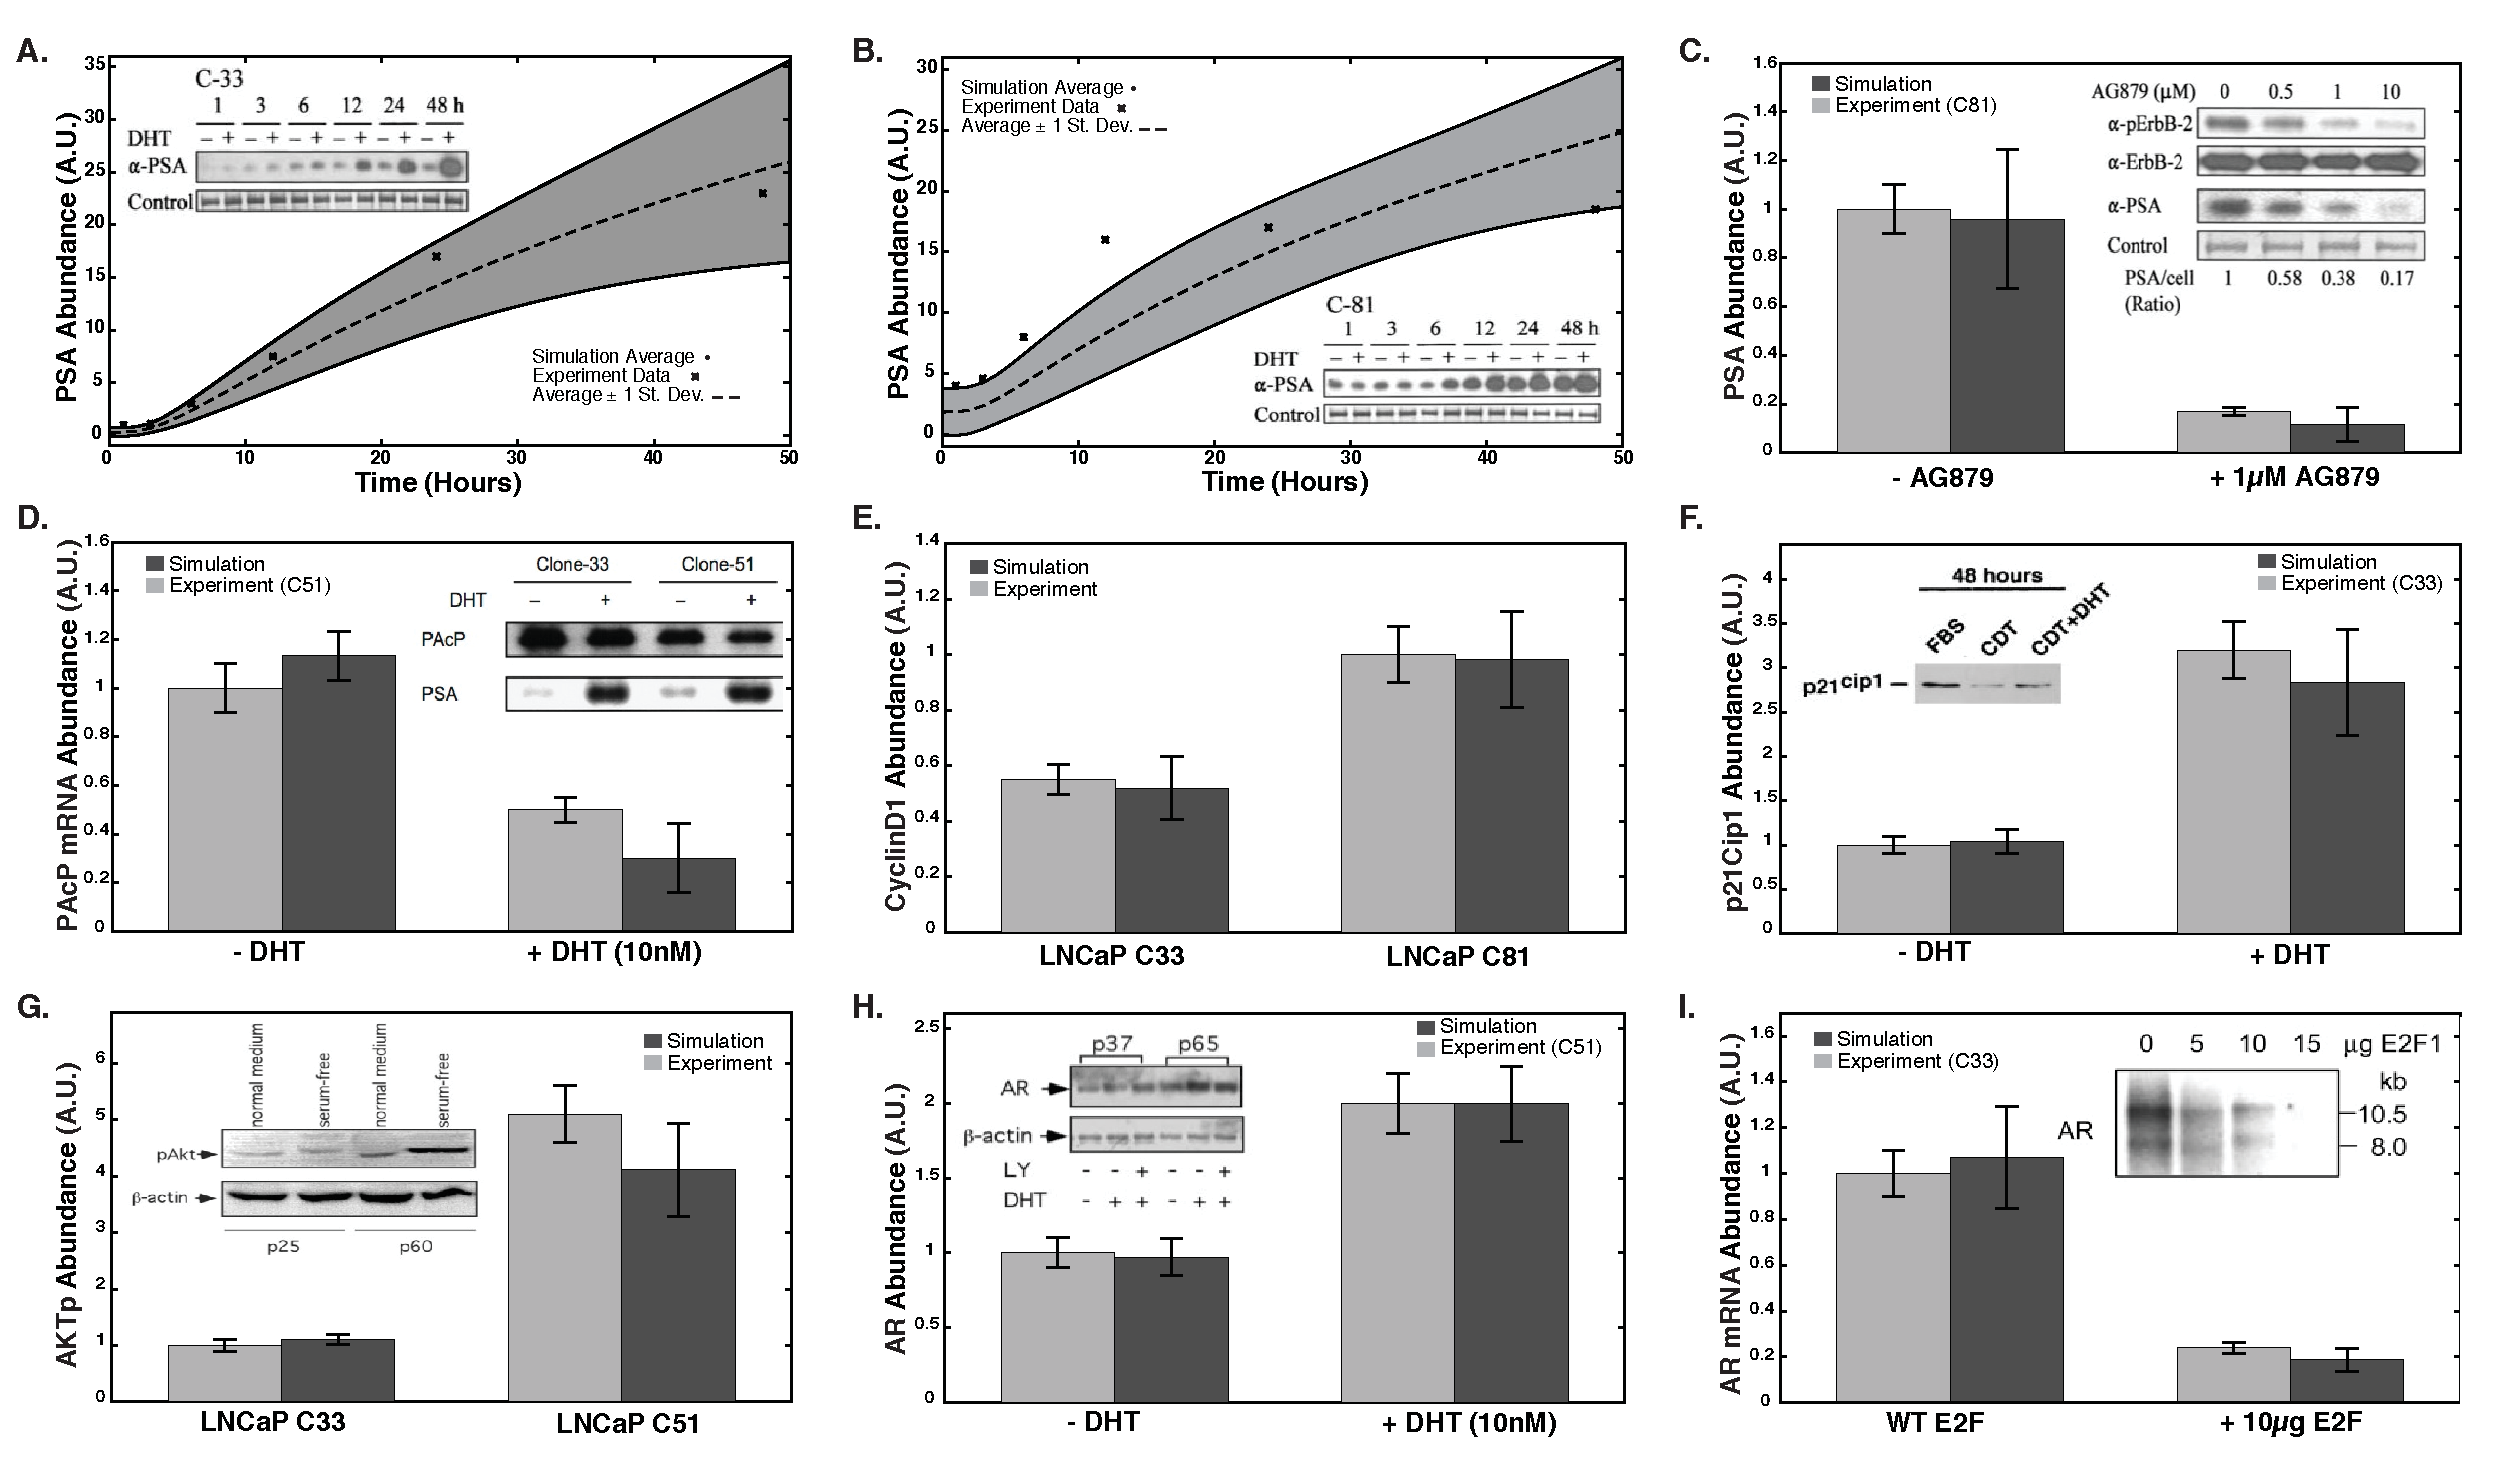
\includegraphics[width=1.0\textwidth]{./figs/Fig_2_Training.pdf}
\caption{Ensemble performance against selected training objectives (N = 5000). A, B. Time course data for PSA concentration due to a stimulus of 10 nM DHT in LNCaP C33 cells and LNCaP C81 cells, respectively (O2, O3). C. PSA levels in the presence and absence of a HER2 inhibitor (LNCaP C81 cells, O7). D. PAcP mRNA levels at 72 hours in the presence and absence of DHT (LNCaP C51 cells, O14). E. Steady-state cyclin D levels in LNCaP C33 vs. C81 (O17). F. p21Cip1 levels at 48 hrs in the presence and absence of DHT (LNCaP C33, O25). G. Steady-state AKT phosphorylation levels in LNCaP C33 vs. C51 (O30). H. AR levels at 24 hours in the presence and absence of DHT (LNCaP C51, O31). I. AR mRNA levels in the presence and absence of E2F over expression (LNCaP C33, O34).}
\label{fg:Training}
\end{figure}

\clearpage

\begin{figure}\centering
\includegraphics[width=1.0\textwidth]{./figs/Fig_4_Validation.pdf}
\caption{Blind model predictions for the ensemble (N = 5000). The model ensemble’s predictive ability was assessed by comparing simulation versus experimental data not used for training. A. Time course data for HER phosphorylation due to a stimulus of 10 nM DHT (LNCaP C33, P1). B. ERK phosphorylation levels in the presence and absence of a PAcP inhibitor (LNCaP C33 cells, P3). C. AR levels at 24 hrs in varying levels of DHT (LNCaP C33, P17). D. Shc phosphorylation levels at 24 hrs in the presence and absence of DHT (LNCaP C33, P22). E. Time course data for HER phosphorylation due to a stimulus of 1.6 nM EGF (LNCaP C33, P7). F. AR levels in varying levels of EGF (LNCaP C33, P14). G, H, I. Fold change in PSA concentration due to drug stimulus: enzalutamide, lapatinib, and sorafenib.}
\label{fg:Validation}
\end{figure}

\clearpage

\begin{figure}\centering
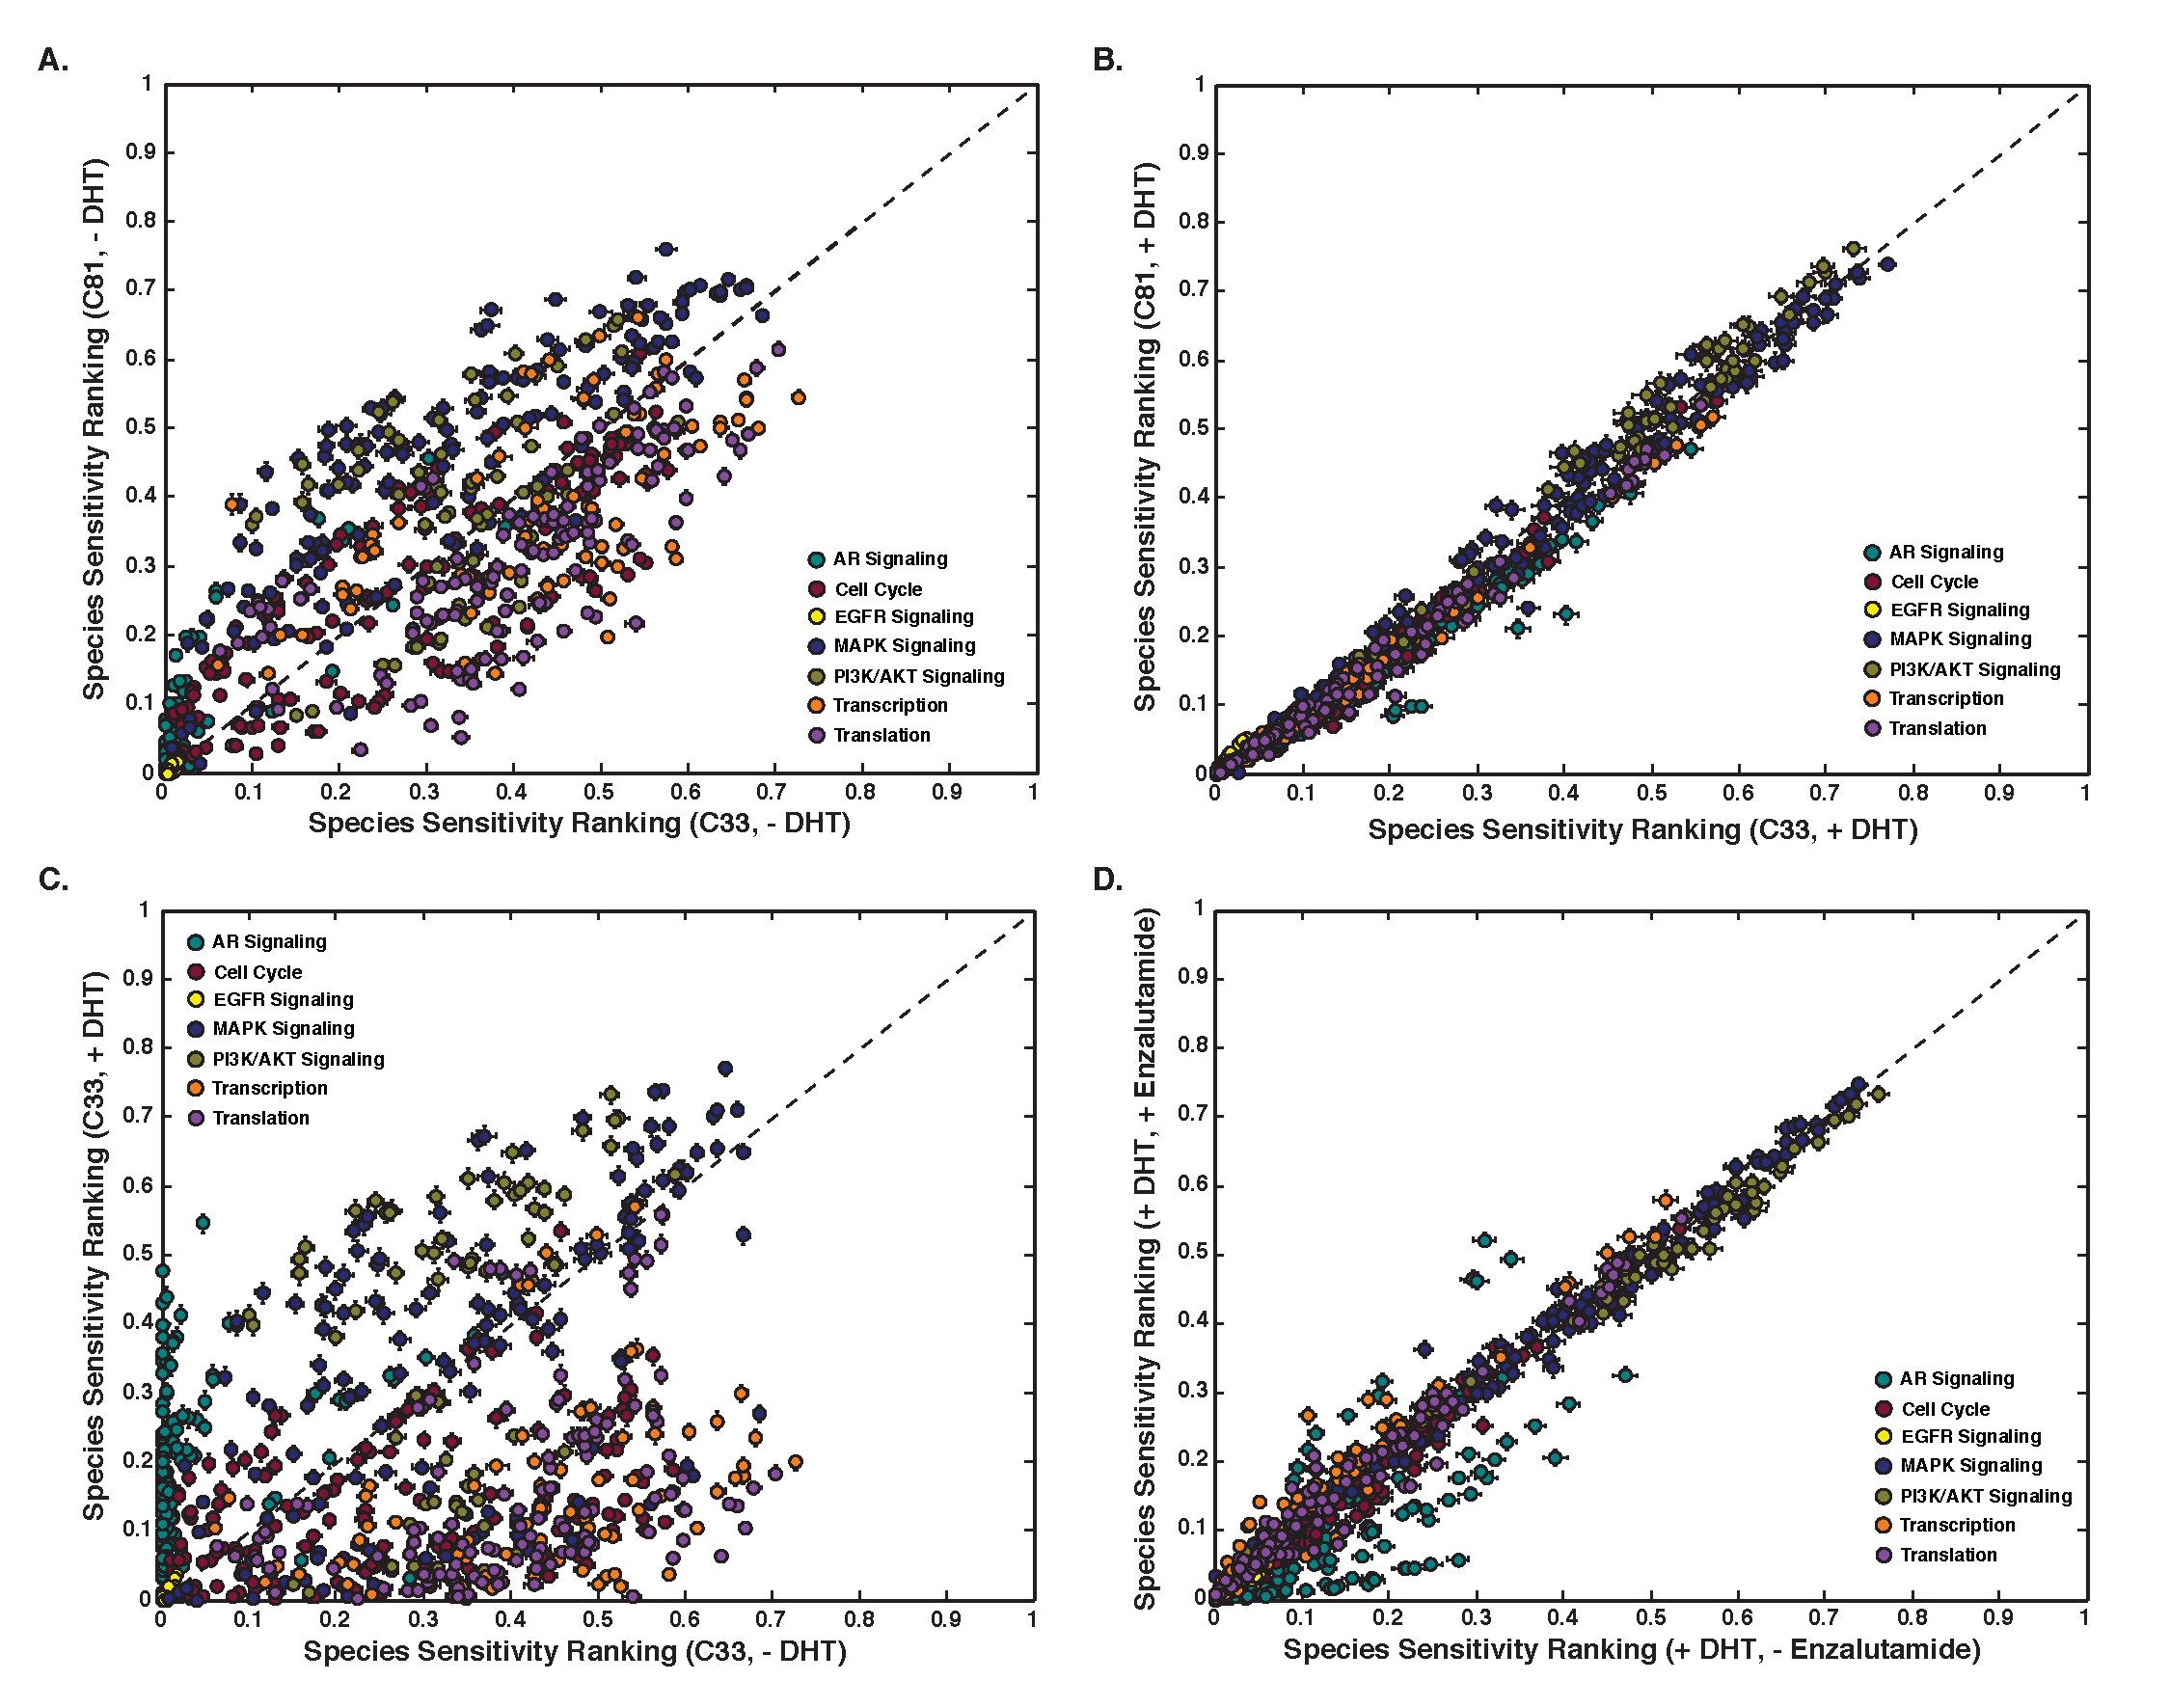
\includegraphics[width=1.0\textwidth]{./figs/Fig_5_Sensitivity.pdf}
\caption{Sensitivity analysis of a population of prostate models (N = 500). Species with a low sensitivity are considered robust, while species with a high sensitivity ranking are considered fragile. $\bf{A,B.}$ Sensitivity ranking of network species in AD versus CR cells in the absence (presence) of DHT. $\bf{C.}$ Sensitivity ranking of network species in AD cells in the absence and presence of DHT. $\bf{D.}$ Sensitivity ranking of network species in CR cells in the presence and absence of enzalutamide with a DHT stimulus.}
\label{fg:Sensitivity}
\end{figure}

\clearpage

\begin{figure}\centering
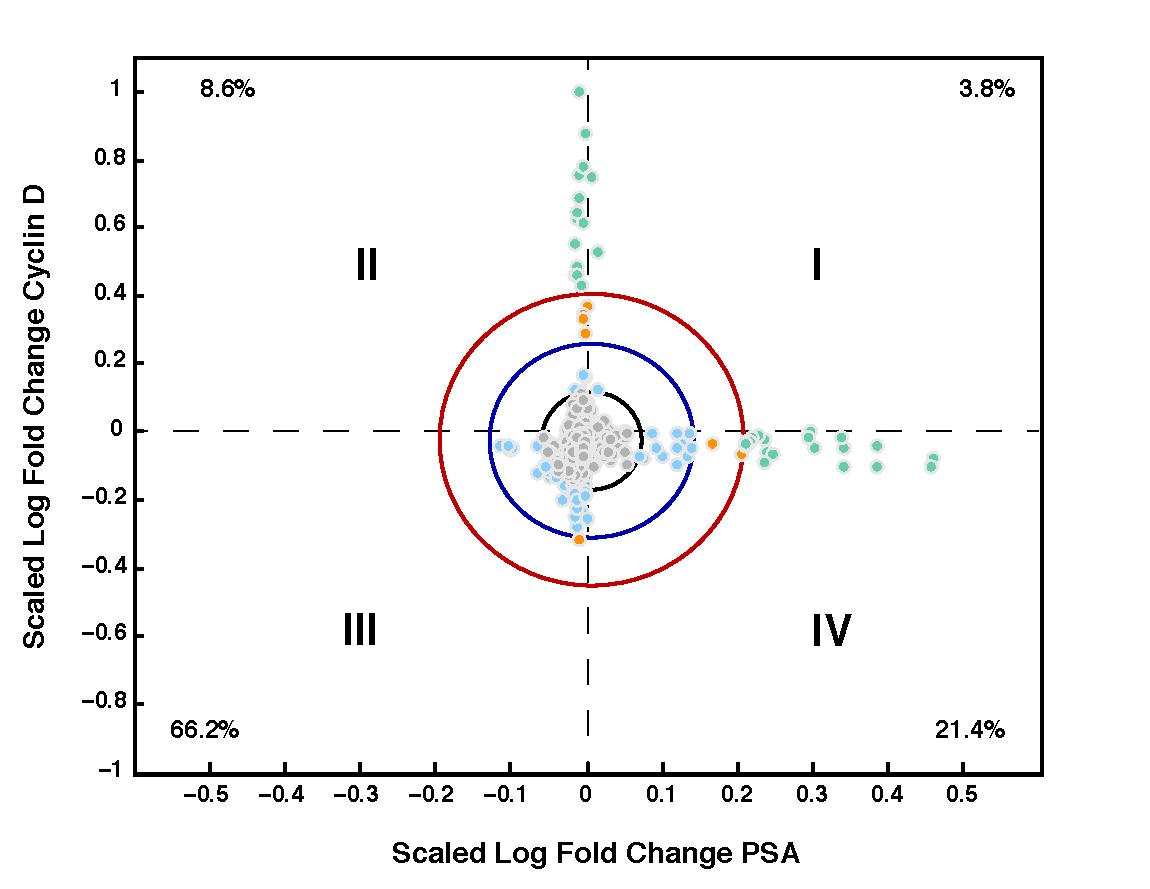
\includegraphics[width=1.0\textwidth]{./figs/Figure6_RAF_K0_C81.pdf}
\caption{Robustness analysis of a population of CR prostate models with Raf knock-out (N = 500). A log fold change of greater then zero implies that the concentration of the protein increased with the knock-out of Raf, while a log fold change of less then zero indicates that the concentration of protein decreased. A log of fold change equal to 0, shows no response due to Raf knock-out. Three distinct regions emerge in Raf knock-out case: (1) PSA increases, (2) cyclin D concentration increases, and (3) PSA and cyclin D concentration decrease. }
\label{fg:Robustness}
\end{figure}

\clearpage

\begin{figure}\centering
\includegraphics[width=1.0\textwidth]{./figs/Figure7_ExperimentalResults.pdf}
\caption{Experimental results for multiple drug combinations on two prostate cancer cell lines, LNCaP and C4-2. A. Western blot analysis of AR, pS6, AKT, pAKT and ERK in LNCaP and C4-2 cell lines treated for 24 hrs with DMSO (control), sorafenib (5 $\mu$M), LY294002 (40 $\mu$M), and MDV3100 (10 $\mu$M) alone or in combination (at least 3 repeats). B. Cells (LNCaP and C4-2) were treated for 24, 48 and 72 hrs with sorafenib (5 $\mu$M), LY294002 (40 $\mu$M), and MDV3100 (10 $\mu$M) and cell viability was measured using MTT Assay. Values were normalized to DMSO (control). C. Cell viability results for LNCaP and C4-2 cells at varying concentration of sorafenib, LY294002, and MDV3100 after 24 hrs of treatment. Values were normalized to DMSO (control). Error bars represent standard error (at least 3 repeats with triplicates performed in each experiment).}
\label{fg:Experiment}
\end{figure}

\clearpage

% Supplemental figures -
% Set the S- 
\renewcommand\thefigure{S\arabic{figure}}
\renewcommand\thetable{T\arabic{table}}
\renewcommand\thepage{S-\arabic{page}}
\renewcommand\theequation{S\arabic{equation}}

% Reset the counters -
\setcounter{equation}{0}
\setcounter{table}{0}
\setcounter{figure}{0}
\setcounter{page}{1}

\section*{Supplementary materials}

\subsection*{Estimation of a population of models using Pareto Optimal Ensemble Techniques (POETs).}

We used multiobjective optimization to estimate an ensemble of prostate models. Although computationally more complex than single-objective formulations, multiobjective optimization can be used to address qualitative conflicts in training data arising from experimental error or cell-line artifacts \cite{Handl2007}. In this study we used the Pareto Optimal Ensemble Technique (POETs) to perform the optimization. POETs integrates standard search strategies, e.g., Simulated Annealing (SA) or Local Pattern Search (PS) with a Pareto-rank fitness assignment \cite{Song2010}. The mean squared error, $\eta$, of parameter set $\mathbf{k}$ for training objective $j$ was defined as:    

\begin{equation}
\eta_j(\mathbf{p}_k) = \frac{1}{N}\sum_{i}^{N}\frac{(\hat{x}_{i,j} - \beta_j x(\mathbf{p_k})_{i,j})^2}{\hat{\sigma}^2_{i,j}}
\end{equation}
The symbol $\hat{x}_{i,j}$ denotes scaled experimental observations (from training objective j) while $x(\mathbf{p_k})_{i,j}$ denotes the simulation output (from training objective j). The quantity $i$ denotes the sampled time-index or condition, and $N$ denotes the number of time points or conditions for experiment j. The standard deviation, $\hat{\sigma}_{i,j}$, was assumed to be equal to 10\% of the reported observation, if no experimental error was reported. $\beta_j$ is a scaling factor which is required when considering experimental data that is accurate only to a multiplicative constant. In this study, the experimental data used for training and validation was typically band intensity from immunoblots, where intensity was estimated using the ImageJ software package \cite{Abramoff2004}. The scaling factor used was chosen to minimize the normalized squared error \cite{Brown2003}:

\begin{equation}
\beta_j = \frac{\sum_{i}(\hat{x}_{i,j}x_{i,j}/\hat{\sigma}_{i,j}^2)}{\sum_{i}(x_{i,j}/\hat{\sigma}_{i,j})^2}
\end{equation} 
By using the scaling factor, the concentration units on simulation results were arbitrary, which was consistent with the arbitrary units on the experimental training data. All simulation data was scaled by the corresponding $\beta_j$. 

We computed the Pareto rank of parameter set $\mathbf{k}_{i+1}$ by comparing the simulation error at iteration $i+1$ against the simulation archive, denoted as $\mathbf{K}_i$. We used the Fonseca and Fleming ranking scheme \cite{Fonseca1993} to estimate the rank of the parameter set $\mathbf{k}_{i+1}$. Parameter sets with increasing rank are progressively further away from the optimal trade-off surface. The parameter set $\mathbf{k}_{i+1}$ was accepted or rejected by the SA with probability $\mathcal{P}\left(\mathbf{k}_{i+1}\right)$: 
\begin{equation}\label{eqn_costMOSA}
\mathcal{P}(\mathbf{k}_{i+1}) \equiv \exp{\{-rank\left(\mathbf{k}_{i+1} \mid \mathbf{K}_{i} \right)/T\}}
\end{equation}
where $T$ is the computational annealing temperature. The Pareto rank for $\mathbf{k}_{i+1}$ is denoted by $rank\left(\mathbf{k}_{i+1}\mid \mathbf{K}_{i}\right)$. The annealing temperature was  adjusted according to the schedule
$T_k = \beta^k T_0$
where $\beta$ was defined as $\beta = \left(\frac{T_{f}}{T_{o}}\right)^{1/10}$. The initial temperature was given by $T_0 = n/log(2)$, with $n=4$ and the final temperature $T_f = 0.1$ used in this study.
The epoch-counter $k$ was incremented after the addition of 50 members to the ensemble. As the ensemble grew, the likelihood of accepting a high rank set decreased. Parameter sets were generated by applying a random perturbation in log space: 

\begin{equation}
\log\mathbf{k}_{i+1} = \log\mathbf{k}_i + \mathcal{N}(0,\nu)
\end{equation}
where $\mathcal{N}(0,\nu)$ is a normally distributed random number with zero mean and variance $\nu$, set as 0.1 in this model. The perturbation was applied in log space to account for large variation in parameter scales and to ensure positive parameter values. We used a local pattern search every $q$ steps, in our case 20, to minimize error for a single randomly selected objective. The local pattern-search algorithm used has been described previously \cite{Gadkar2003}.

%! program = pdflatex

%\documentclass[12pt]{article}
%\usepackage{geometry} % see geometry.pdf on how to lay out the page. There's lots.
%\geometry{a4paper} % or letter or a5paper or ... etc
% \geometry{landscape} % rotated page geometry

% See the ``Article customise'' template for come common customisations

%\usepackage{supertabular}


%*** extra packages ****
%\usepackage{colortbl}
%\usepackage{color}
%\usepackage{amsmath}
%\usepackage{amssymb}
%\renewcommand{\rmdefault}{phv}\renewcommand{\sfdefault}{phv}
%\textwidth = 7.5 in
%\textheight = 9.75 in
%\oddsidemargin = 0.0 in
%\evensidemargin = 0.0 in
%\topmargin = 0.01 in
%\headheight = 0.0 in
%\headsep = 0.25 in
%\hoffset = -0.5 in
%\begin{document}

\begin{center}
\tablefirsthead{
\hline
\rowcolor[gray]{0.8}\textbf{O\#}  & \textbf{Species} & \textbf{Cell~Type} & \textbf{Stimulus} & \textbf{SS or D} & \textbf{Source} \\
\hline}
\topcaption{Objective function list along with species measured, 
  stimulus, cell-type, steady state (SS) vs dynamic (D) and the
  corresponding literature reference.}
\label{objective_table}
\begin{scriptsize}
\begin{supertabular}{l l l l l l l l l }  
\hline \\ 												
O1  & PSA & C33/C81 & 0  & SS & \cite{Lee2003} \\
O2  & PSA & C33 & DHT & D & \cite{Lee2003} \\
O3  & PSA & C81 & DHT & D &  \cite{Lee2003} \\
O4  & ERK-p & C33 & DHT & D &  \cite{Lee2003} \\
O5  & ERK-p & C81 & DHT & D & \cite{Lee2003} \\
O6  & PSA & C33 & HER2 Knockdown & SS & \cite{Lee2003} \\
O7  & PSA & C81 & HER2 Knockdown & SS & \cite{Lee2003} \\
O8  & PSA & C33 & MEK Up & SS & \cite{Lee2003} \\
O9  & PSA & C81 & MEK Down & SS & \cite{Lee2003} \\
O10  & PSA & C33 & HER2 Up & SS & \cite{Lee2003} \\
O11  & ERK-p & C33 & HER2 Up & SS & \cite{Lee2003} \\
O12  & AR & C33/C51/C81 & 0 & SS & \cite{Lin2000} \\
O13  & PAcP mRNA & C33 & DHT & D & \cite{Lin2000} \\
O14  & PAcP mRNA & C51 & DHT & D & \cite{Lin2000} \\
O15  & PAcP mRNA & C81 & DHT & D & \cite{Lin2000} \\
O16  & HER2-p & C33/C51/C81 & 0 & SS & \cite{Yuan2007} \\
O17  & Cyclin D & C33/C81 & 0 & SS & CITE \\
O18  & Cyclin D & C33 & EGF & D &  \cite{Perry1998}\\
O19  & Cyclin D mRNA & C33 & EGF & D &  \cite{Perry1998}\\
O20  & AKT-p & C51/LNCaP-Rf  & 0 & SS & \cite{Murillo2001}\\
O21  & p27Kip1 & C51/LNCaP-Rf  & 0 & SS & \cite{Murillo2001}\\
O22  & p21Cip1 & C51/LNCaP-Rf  & 0 & SS & \cite{Murillo2001}\\
O23  & Rb-p & C33 & DHT & D & \cite{Xu2006}\\
O24  & p70-p & C33 & DHT & D & \cite{Xu2006}\\
O25  & p21Cip1 & C33 & DHT & D & \cite{Knudsen1998}\\
O26  & p27Kip1 & C33 & DHT & D & \cite{Knudsen1998}\\
O27  & PSA mRNA & C33 & Cyclin E Up + DHT & D & \cite{Yamamoto2000}\\
O28  & AR mRNA & C33 & Cyclin E Up + DHT & D & \cite{Yamamoto2000}\\
O29  & PSA mRNA & C33 & HER2 Up & SS & \cite{Yeh1999}\\
O30  & AKT-p & C33/C51 & 0 & SS & \cite{Lin2003}\\
O31  & AR & C51 & DHT & D & \cite{Lin2003}\\
O32  & AR & C33 & DHT & D & \cite{Chen2009}\\
O33  & Cyclin D1b mRNA & C33 & Sam68 Knockdown & SS & \cite{Paronetto2010}\\
O34  & AR mRNA & C33 & E2F Up & SS & \cite{Davis2006}\\
O35  & AR & C33 & E2F Up & SS & \cite{Davis2006}\\
O36  & AR Cyclin E & C33 & E2F Up & SS & \cite{Davis2006}\\
O37  & PSA & C33 & E2F Up & SS & \cite{Davis2006}\\
O38  & cPAcP & C33 & DHT & D & \cite{Meng2000}\\
O39  & Cyclin D & C33 & DHT & D &  \cite{Xu2006}\\
O40  & 4EBP1-p & C33 & DHT & D &  \cite{Xu2006}\\
O41*  & PAcP mRNA & C33/C51/C81 & 0 & SS & \cite{Lin2000} \\
O42*  & p16INK4 & C51/C81 & 0 & SS & \cite{Murillo2001}\\
O43*  & cPAcP & C33/C51/C81 & 0 & SS & \cite{Lin2001}\\


\end{supertabular}
\end{scriptsize}
\end{center}
%\end{document}
 
 

 
 
 
 
 
 
 
 

  
 
  
   


 
 
 
 
 
 
 
 
 
 
 
 
 
 
 
 
 

\clearpage

%! program = pdflatex

%\documentclass[12pt]{article}
%\usepackage{geometry} % see geometry.pdf on how to lay out the page. There's lots.
%\geometry{a4paper} % or letter or a5paper or ... etc
% \geometry{landscape} % rotated page geometry

% See the ``Article customise'' template for come common customisations

%\usepackage{supertabular}


%*** extra packages ****
%\usepackage{colortbl}
%\usepackage{color}
%\usepackage{amsmath}
%\usepackage{amssymb}
%\renewcommand{\rmdefault}{phv}\renewcommand{\sfdefault}{phv}
%\textwidth = 7.5 in
%\textheight = 9.75 in
%\oddsidemargin = 0.0 in
%\evensidemargin = 0.0 in
%\topmargin = 0.01 in
%\headheight = 0.0 in
%\headsep = 0.25 in
%\hoffset = -0.5 in
%\begin{document}

\begin{center}
\tablefirsthead{
\hline
\rowcolor[gray]{0.8}\textbf{Prediction\#}  & \textbf{Species} & \textbf{Cell~Type} & \textbf{Stimulus} & \textbf{SS or D} & \textbf{Source} \\
\hline}
\topcaption{Blind Prediction list along with species measured, 
  stimulus, cell-type, steady state (SS) vs dynamic (D) and the
  corresponding literature reference.}
\label{prediction_table}
\begin{scriptsize}
\begin{supertabular}{l l l l l l l l l }  
\hline \\ 												

P1 & HER2-p & C33 & DHT  & D & \cite{Meng2000} \\
P2  & p27Kip1 & C33 & SHP Knockdown  & D & \cite{Rodriguez-Ubreva2010}\\
P3  & ERK-p & C33 & PAcP Knockdown  & SS &  \cite{Chuang2010}\\
P4  & AKT-p & C33 & PAcP Knockdown  & SS &  \cite{Chuang2010}\\
P5  & Cyclin D1 & C33 & PAcP Knockdown  & SS &  \cite{Chuang2010}\\
P6  & EGFR-p & C33 & EGF  & D & \cite{Chen2011}\\
P7  & HER2-p & C33 & EGF  & D & \cite{Chen2011}\\
P8  & EGFR-p & LNCaP-AI & EGF  & D & \cite{Chen2011}\\
P9  & HER2-p & LNCaP-AI & EGF  & D & \cite{Chen2011}\\
P10  & CyclinE & C33 & DHT  & D & \cite{Knudsen1998}\\
P11  & CDK2 & C33 & DHT  & D & \cite{Knudsen1998}\\
P12  & HER2-p & C33/C81 & 0  & SS & \cite{Chuang2010}\\
P13  & AR & C33 & EGF  & D & \cite{Cai2009}\\
P14  & AR & C33 & EGF  & D & \cite{Cinar2005}\\
P15  & p27Kip1 & C33 & DHT  & D & \cite{Fang2012}\\
P16  & Rb-p & C33 & DHT  & D & \cite{Knudsen1998}\\
P17  & AR & C33 & DHT  & D & \cite{Cai2009}\\
P18  & AKT-p & C33 & DHT  & D & \cite{Cai2009}\\
P19  & PSA & C33 & EGF + DHT  & D & \cite{Cai2009}\\
P20  & PSA & C33 & EGF  & D & \cite{Cai2009}\\
P21  & Cyclin D1 & C33 & Sam68 Knockdown  & SS & \cite{Busa2007}\\
P22  & Shc & C33 & DHT  & D & \cite{Veeramani2005Onc}\\
P23  & Shc & C33 & EGF  & D & \cite{Veeramani2005Onc}\\
P24  & Shc & C33/C81 & 0  & SS & \cite{Veeramani2005Onc}\\
P25  & AR & C33 & AKT-p Knockdown  & SS & \cite{Ha2011}\\
P26  & AR & LNCaP AI & AKT-p Knockdown  & SS & \cite{Ha2011}\\
P27  & 4EBP1 bound eIF4E & C33/LNAI & 0  & SS & \cite{Graff2009}\\
P28  & Shc-p & C33/C51/C81 & 0 & SS & \cite{Lee2004}\\
P29  & Shc-p & C33 & EGF & D & \cite{Lee2004}\\
P30  & PSA Response & CRPC Patients & enzalutamide & D & \cite{Scher2012}\\
P31  & PSA Response & CRPC Patients & sorafenib & D & \cite{Dahut2008}\\
P32  & PSA Response & CRPC Patients & lapatinib & D & \cite{Whang2013}\\
P33  & PSA Response & ADPC Patients & lapatinib & D & \cite{Liu2013}\\

\end{supertabular}
\end{scriptsize}
\end{center}
%\end{document}
 
 

 
 
 
 
 
 
 
 

  
 
  
   


 
 
 
 
 
 
 
 
 
 
 
 
 
 
 
 
 

\clearpage

\begin{figure}\centering
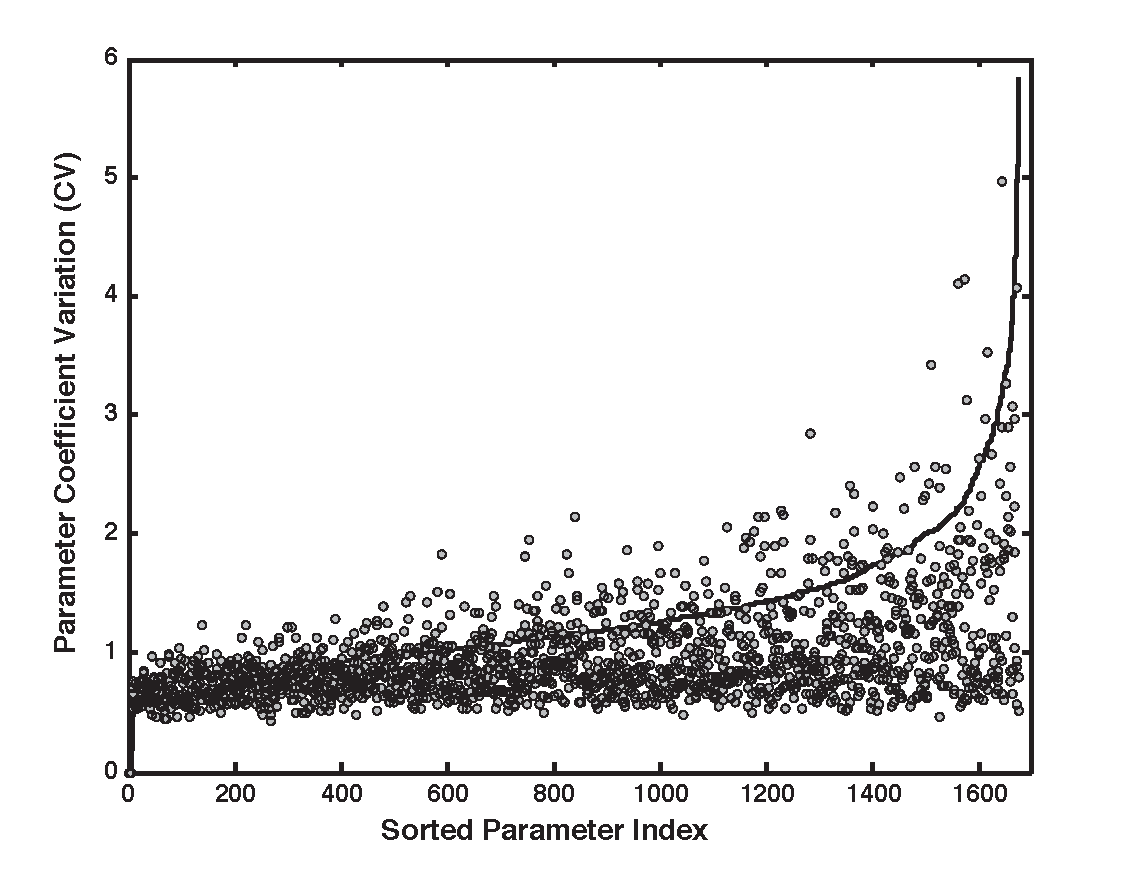
\includegraphics[width=1.0\textwidth]{./figs/Supplementary_CV_Subset_Total}
\caption{Coefficient of variation (CV) of model parameters estimated using POETs. The solid line denotes the mean CV calculated over the entire ensemble (N = 5000). The points denote the mean CV of the 500 ensemble members used for sensitivity and robustness calculations. Over the ensemble, the coefficient of variation (CV) of the kinetic parameters spanned 0.59 - 5.8, with 33\% of the parameters having a CV of less than one.}
\label{fg:Supp_CV}
\end{figure}

\begin{figure}\centering
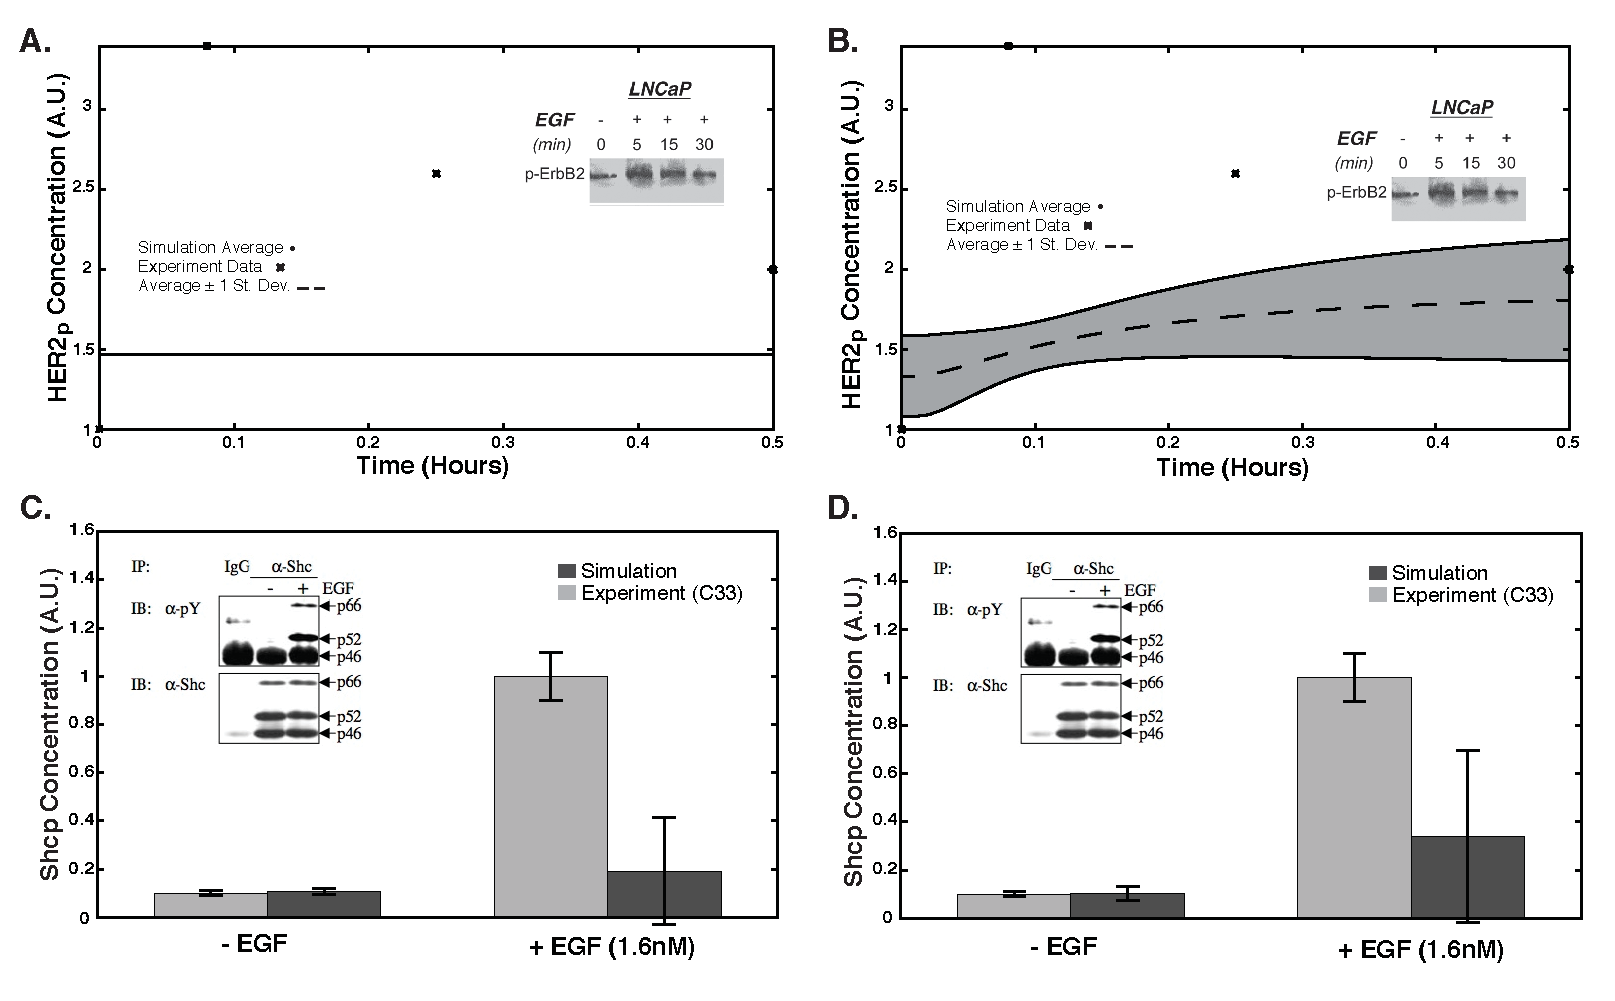
\includegraphics[width=1.0\textwidth]{./figs/Supp_Figure_NewModelvsOldModel}
\caption{Blind model predictions for the ensemble with the original and updated model (EGFR and HER2 heterodimer). A,B. Time course data for HER phosphorylation due to a stimulus of 1.6 nM EGF (LNCaP C33, P7) for the old and new model, respectively. Dark grey shows only parameters improved by the updated model (N=2870) while light grey show all parameter sets (N=5000). C,D. Shc phosphorylation levels at 16 hrs in the presence and absence of 1.6 nM EGF (LNCaP C33, P29) for the old and new model, respectively. Light grey denotes experimental data, mid grey denotes simulation results for all parameters (N=5000), and black denotes only parameters improved by the updated model (N=3142).}
\label{fg:Exps_NewModelvsOldModel}
\end{figure}


\begin{figure}\centering
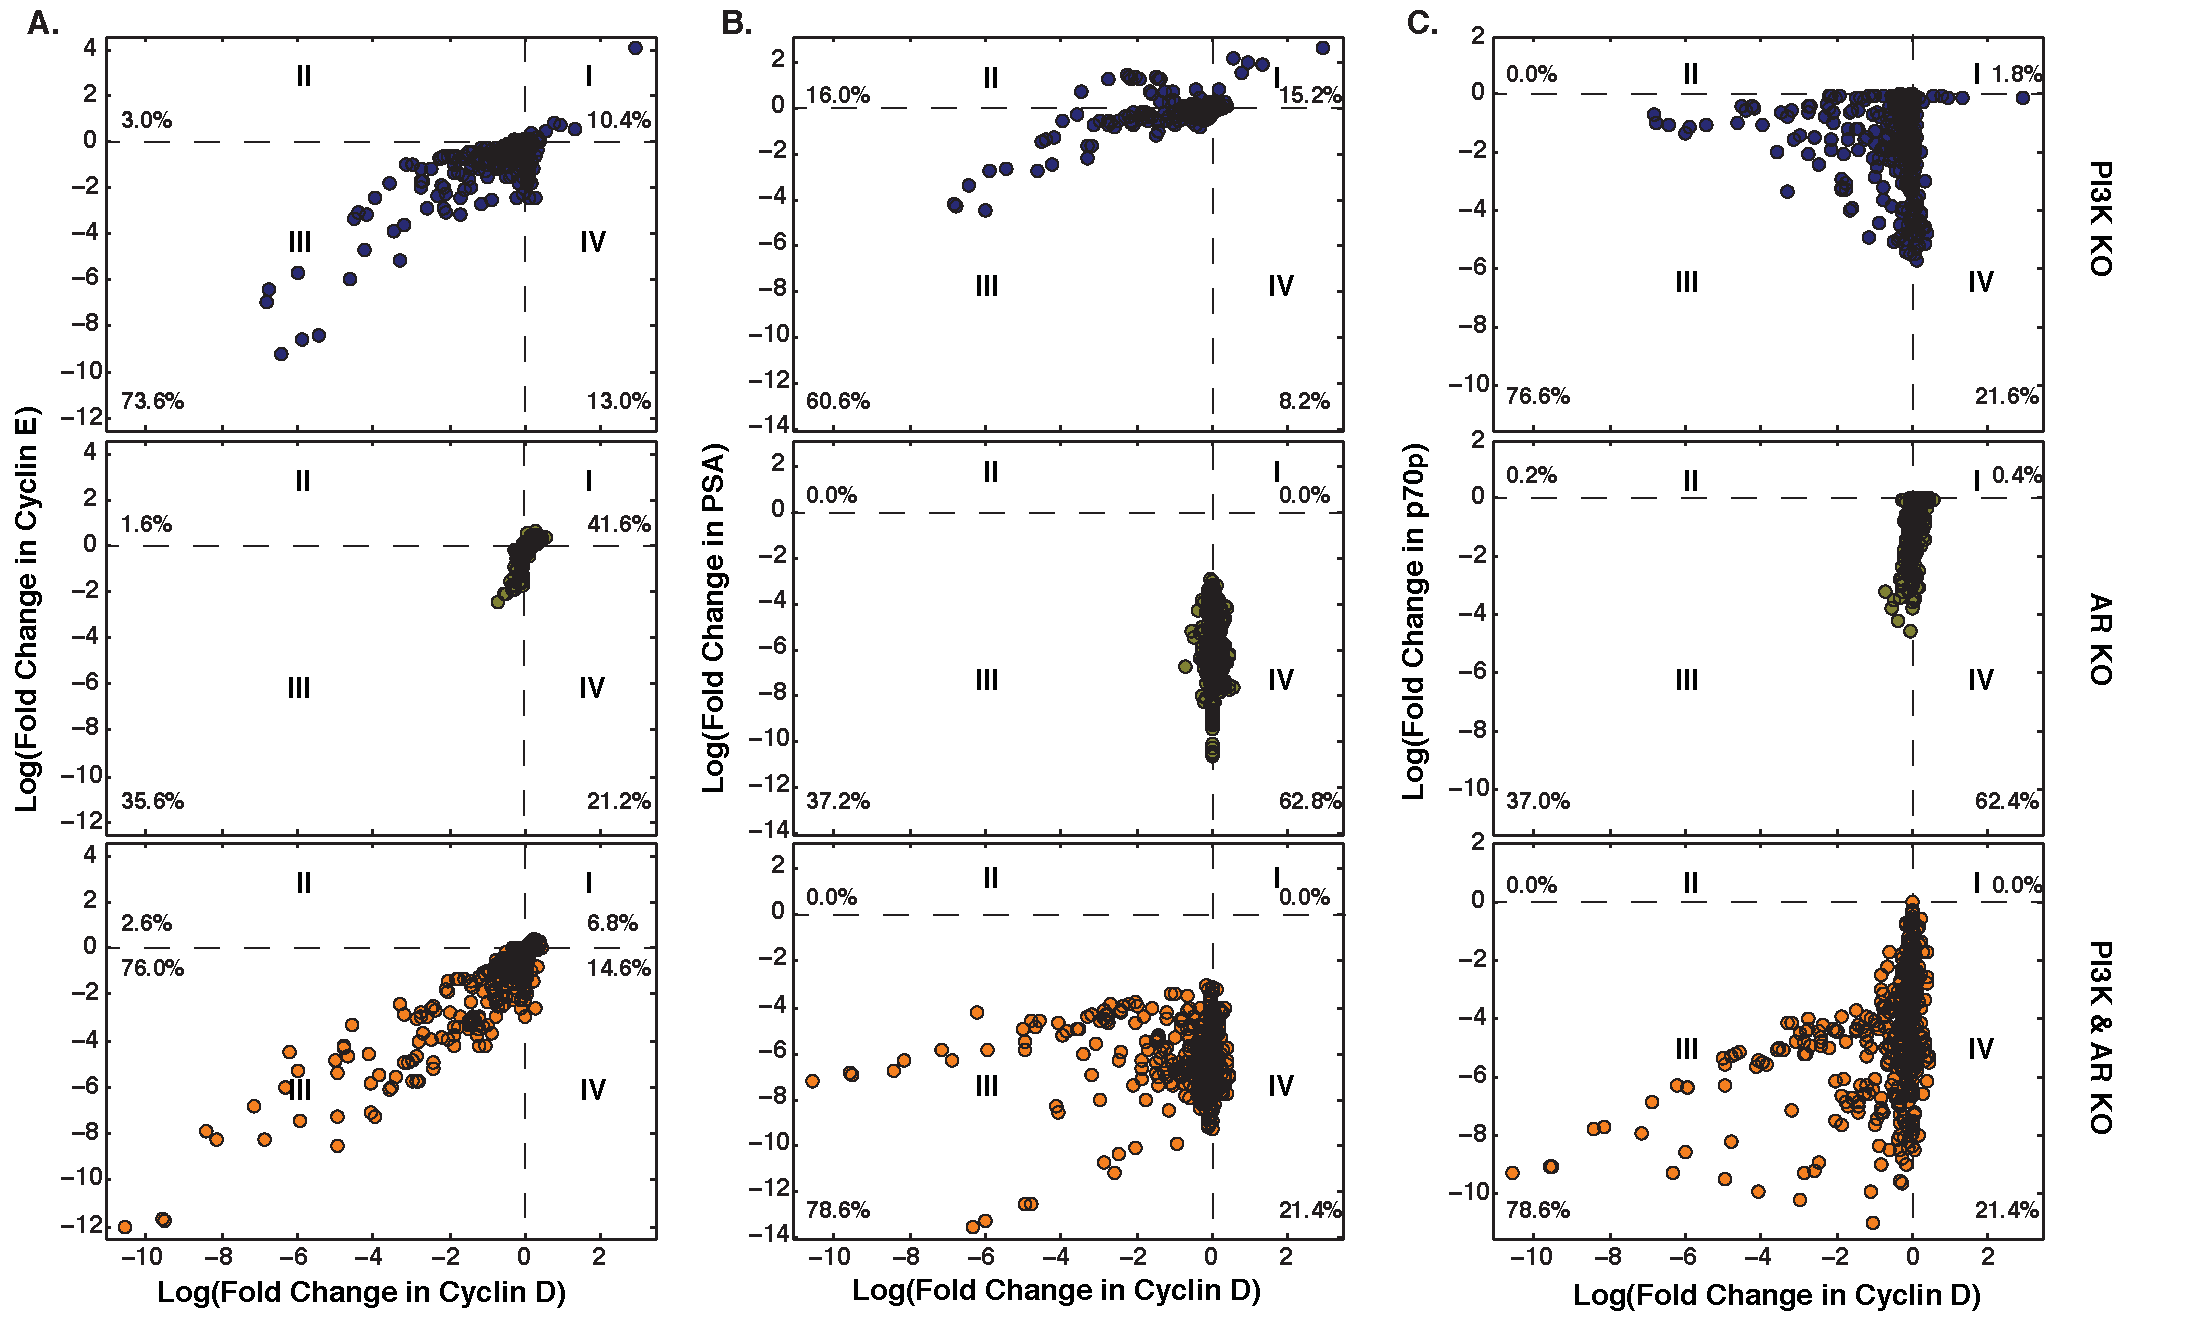
\includegraphics[width=1.0\textwidth]{./figs/Fig_6_PI3K_AR_KO_3_Cases.pdf}
\caption{Robustness analysis of a population of CR prostate models with PI3K (blue), AR (green), and PI3K and AR (orange) knock-outs (N = 500). A log fold change of greater then zero implies that the concentration of the protein increased with the knock-out, while a log fold change of less then zero indicates that the concentration of protein decreased. A log of fold change equal to 0, shows no response due to the knock-out.
 A.,B.,C. Log robustness of cyclin E, PSA, and p70p versus Cyclin D for the three knock-out cases. A CR LNCaP cell was assumed for all knock-out cases.}
\label{fg:Supp_Dual_Knockout}
\end{figure}

\begin{figure}\centering
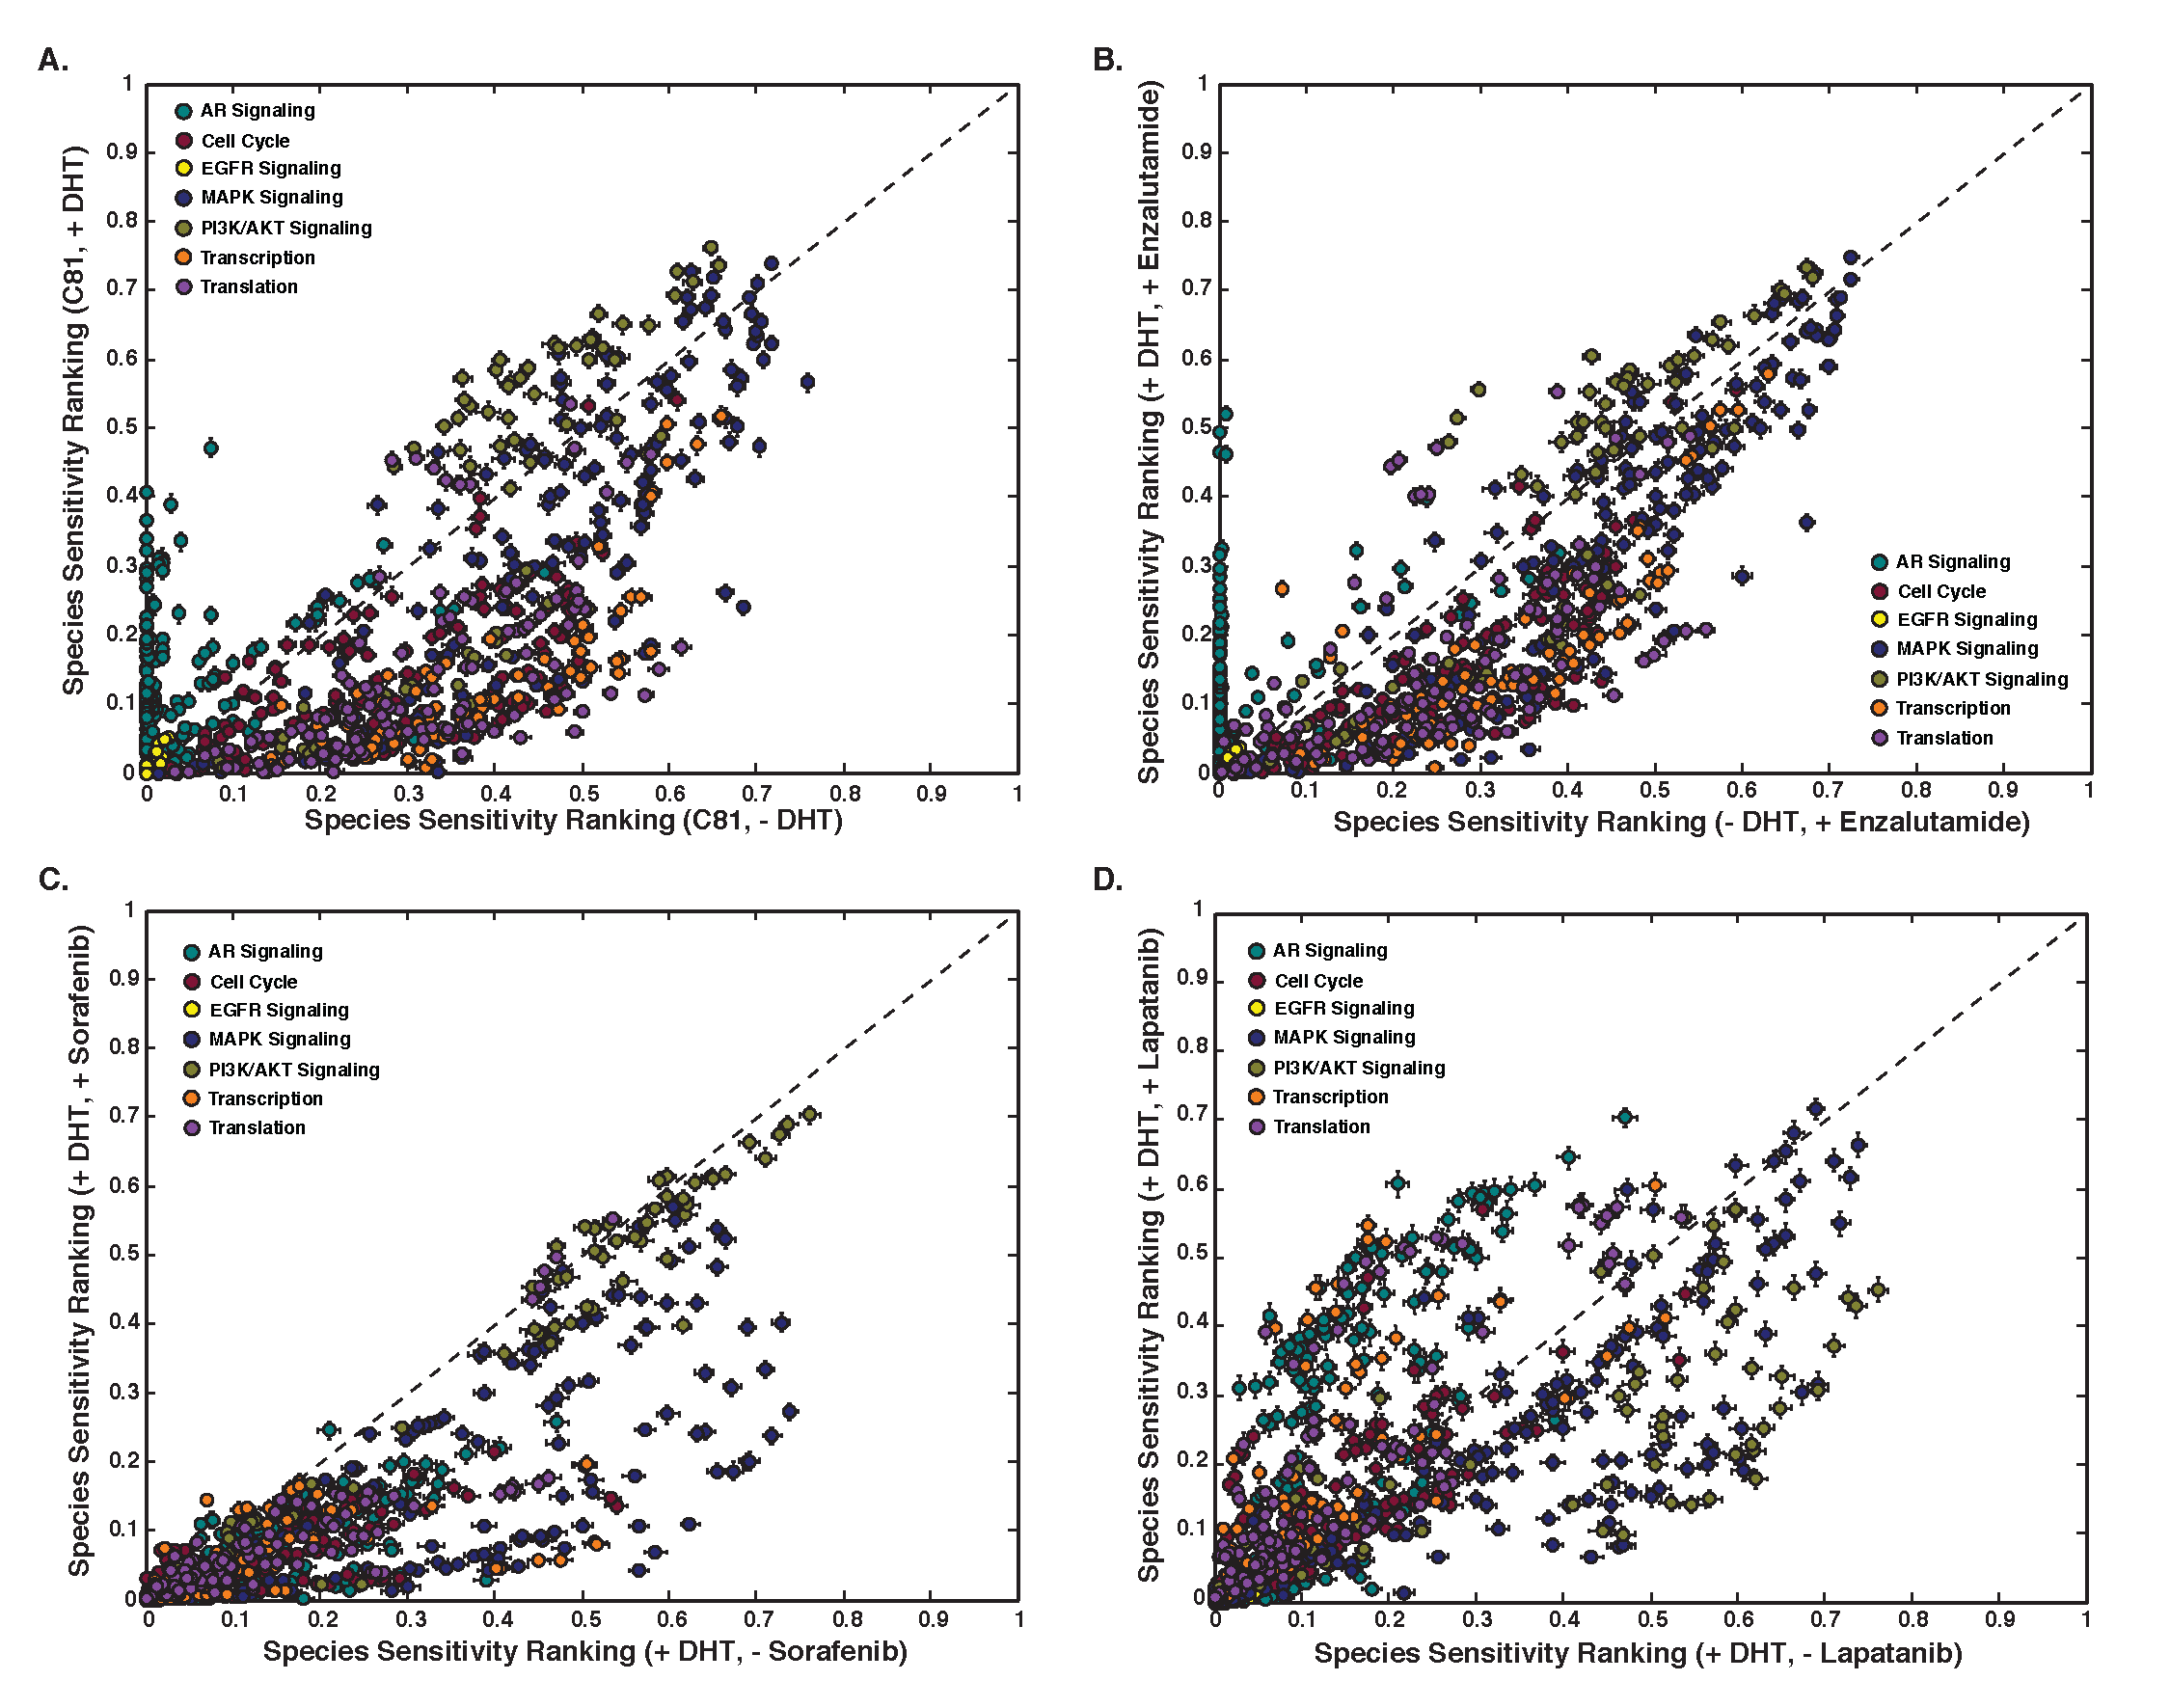
\includegraphics[width=1.0\textwidth]{./figs/Supp_Figure_Sensitivity.pdf}
\caption{Sensitivity analysis of a population of prostate models (N = 500). Species with a low sensitivity are considered robust, while species with a high sensitivity ranking are considered fragile. $\bf{A}$ Sensitivity ranking of network species in CR cells in the absence and presence of DHT. $\bf{B.}$ Sensitivity ranking of network species in CR cells in the presence of enzalutamide in the presence and absence of a DHT stimulus. $\bf{C.,D.}$ Sensitivity ranking of network species in CR cells in the presence and absence of sorafenib and lapatinib, respectively, with a DHT stimulus.}
\label{fg:Supp_Sensitivity}
\end{figure}

\begin{figure}\centering
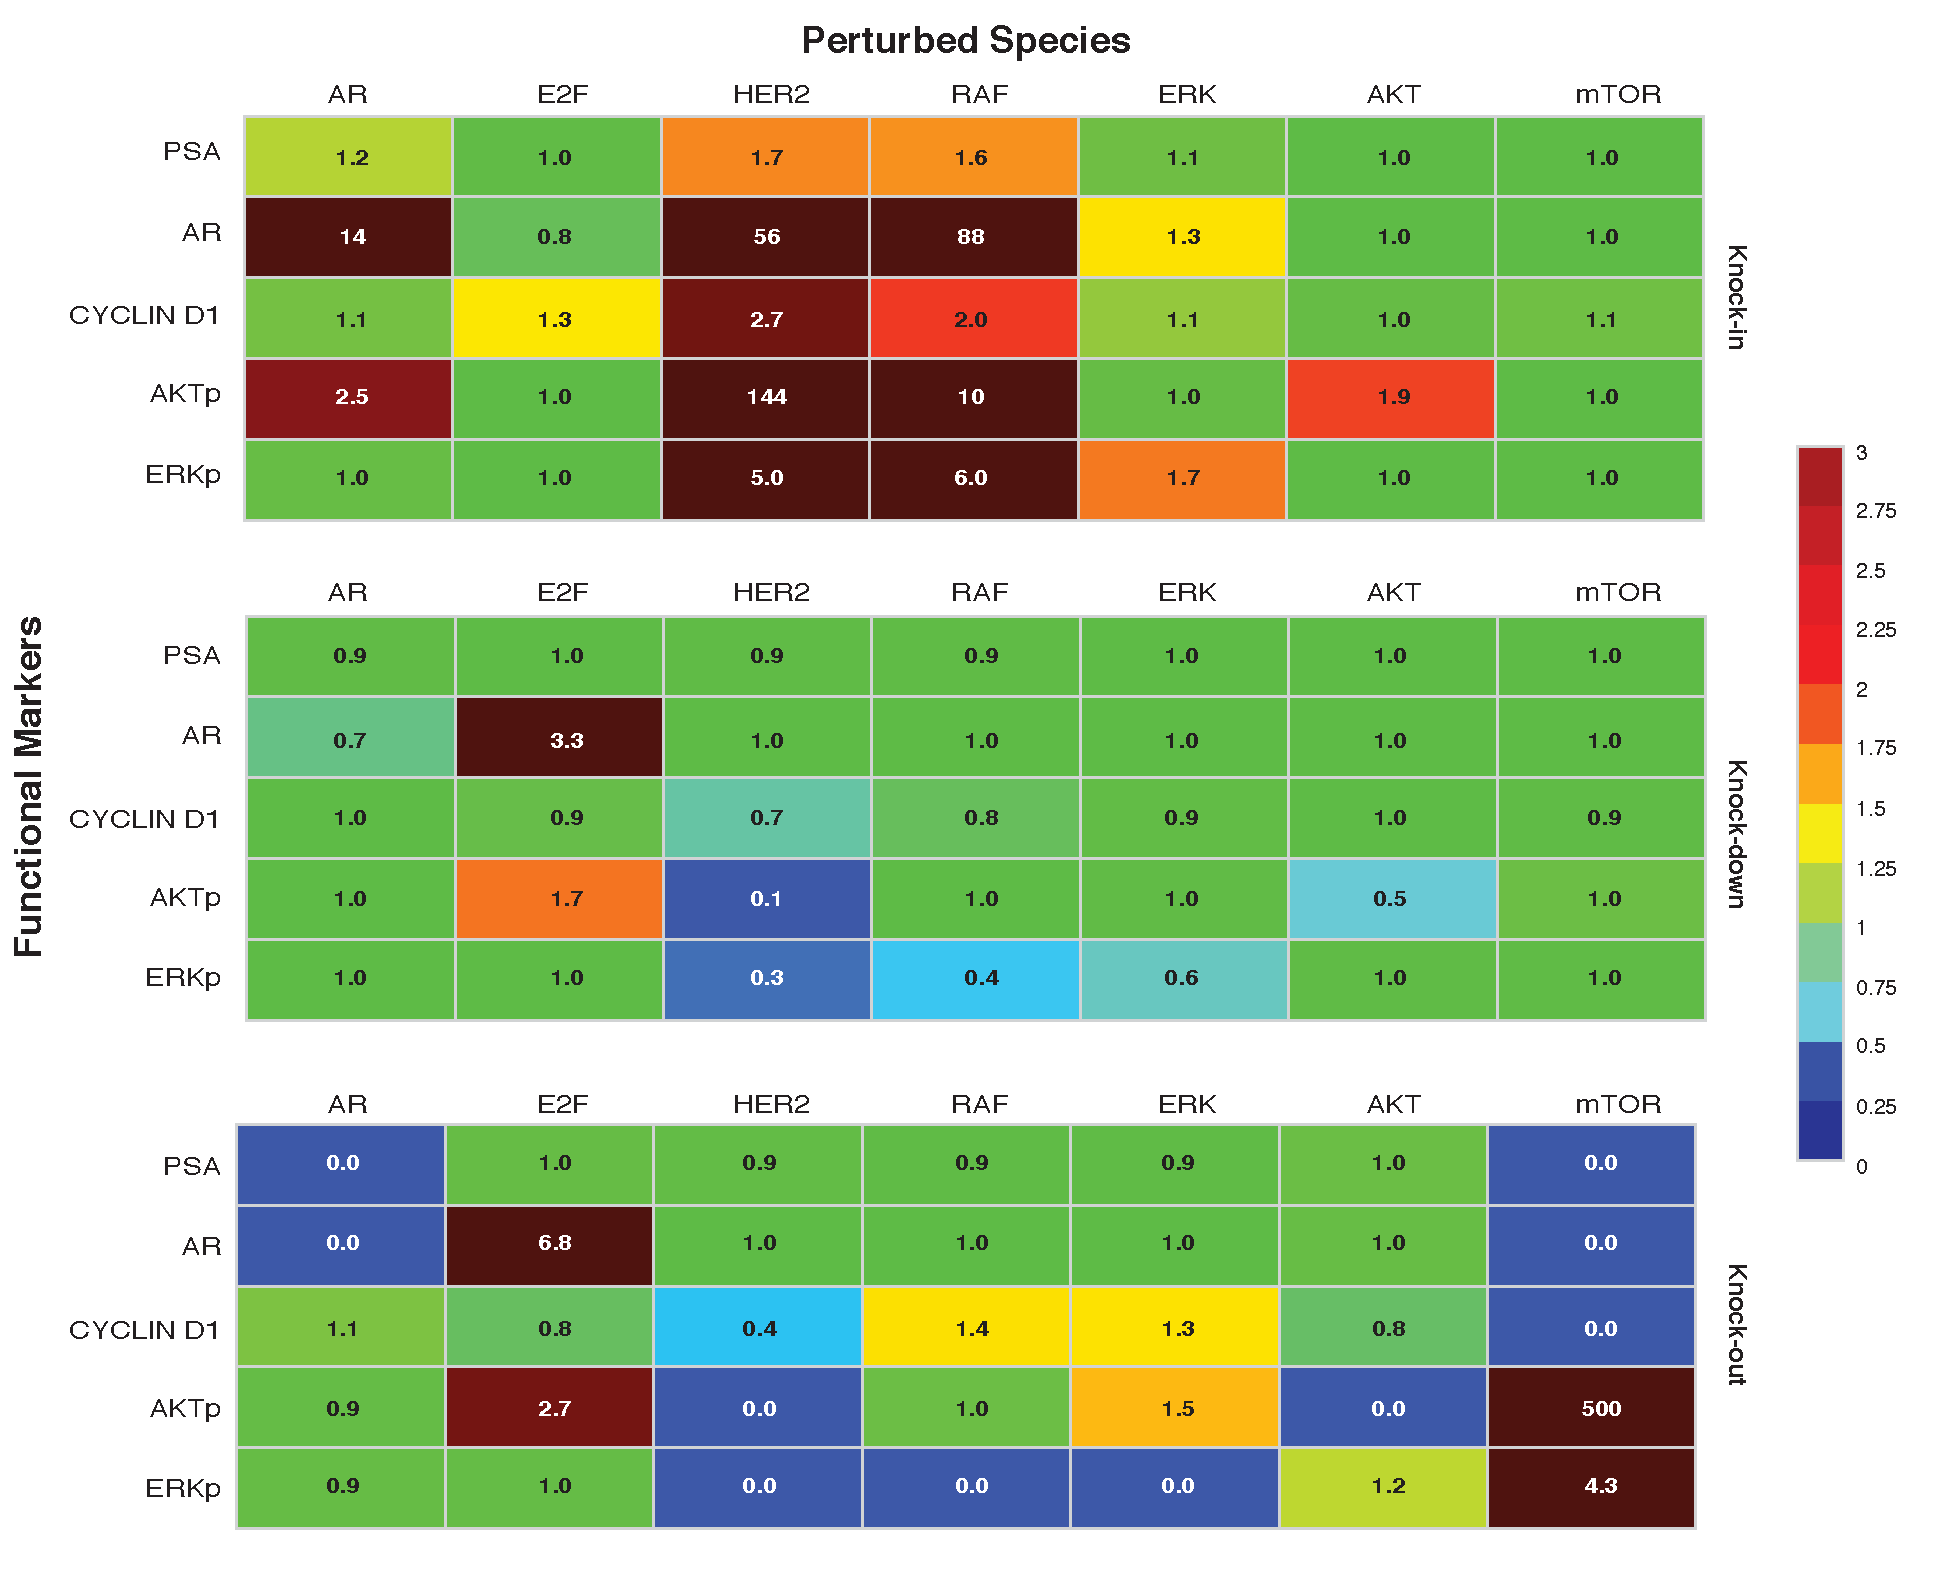
\includegraphics[width=1.0\textwidth]{./figs/Supp_Figure_Robustness.pdf}
\caption{Robustness analysis of protein markers. Expression level of key proteins was altered by a factor of 2, 0.1, or 0 (knock-in, knock-down, or knock-out) and robustness coefficients were calculated for five key protein markers. Simulations shown were from CR cells, with indicated perturbation. Mean of 500 ensemble members is shown.}
\label{fg:Supp_Robustness}
\end{figure}

\begin{figure}\centering
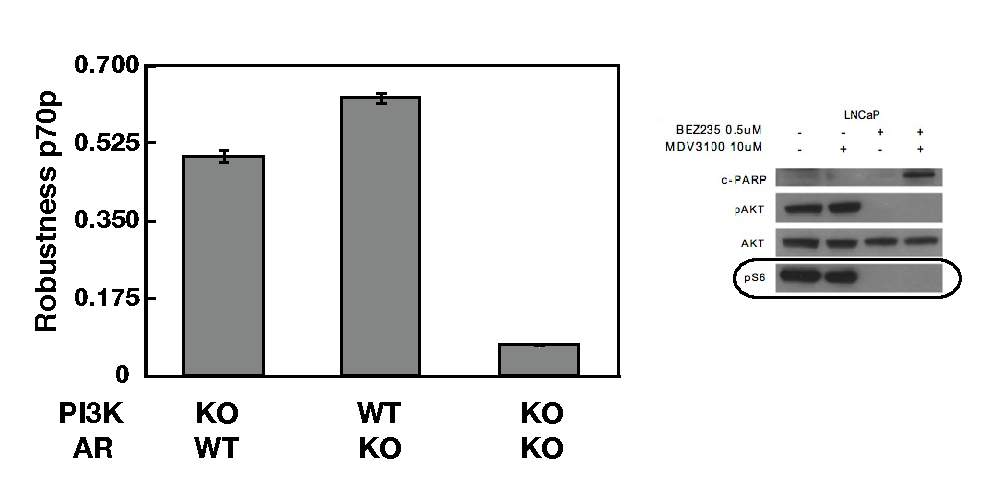
\includegraphics[width=1.0\textwidth]{./figs/Supp_Figure_KO_new.pdf}
\caption{Dual knock-out of AR and PI3K leads to decreased expression of activated p70. A., B, C. Robustness coefficient of activated p70 (S6) in the PI3K knock-out, AR knock-out, and dual knock-out cases, respectively. The control was the basil CR LNCaP wild type case. Error bars denote plus and minus one standard error above the mean with N = 500.  Experimental data is from Carver, et al \cite{Carver2011}.  }
\label{fg:Supp_KO}
\end{figure}

%\end{comment}


\end{document}

